\definecolor{hellgrau}{RGB}{230, 230, 230}
\lohead{Vollmaier Alois}
\chapter{Informatik}\label{ch:informatik}
\section{Allgemeines}\label{sec:einleitung}
Im folgenden Projektteil werden die Kernbestandteile sowie der nähere Aufbau des informatischen Bereichs dieser Arbeit gezeigt.
Weiters werden wesentliche Elemente der Inbetriebnahme der Maschine dokumentiert und zusammengefasst.
Die Aufteilung dieses 55-seitigen Kapitels überstreckt sich über alle signifikanten Teile der grafischen Oberfläche, bezeichnet als \textbf{Frontend}, bis hin zu den im Hintergrund arbeitenden Funktionen, welche als \textbf{Backend} zusammengefasst werden.
Darüber hinaus wird gezeigt, wie Teile der \textbf{hardwarenahen Programmierung} funktionieren und wie diese mit der Steuerelektronik zusammenarbeiten.
Am Schluss wird die Zusammensetzung des \textbf{Teilaufbaus} gezeigt.
\section{Zeitplan}\label{sec:zeitplan}
\begin{figure}[H]
    \centering
    \scalebox{0.57}{
    \begin{ganttchart}[
    hgrid style/.style={black, dotted},
    calendar week text={\currentweek},
    vgrid={*6{white, dotted}, *1{black, dashed}},
    x unit=1mm,
    group label font=\bfseries \Large,
    y unit chart=9mm,
    y unit title=12mm,
    time slot format=isodate,
    time slot unit=year
    link/.style={->, thick}
    ]{2019-09-2}{2020-03-15}
        \gantttitlecalendar{year, month=name, week}\\

        \ganttgroup[
        group/.append style={fill=red}
        ]{Backend-Programmierung}{2019-09-02}{2019-11-15}\\ [grid]
        \ganttbar[
        bar/.append style={pattern=north east lines},
        name=KonzeptplanungBack
        ]{Konzeptplanung}{2019-09-02}{2019-09-25}\\ [grid]
        \ganttbar[
        bar/.append style={pattern=north east lines},
        name=Einrichtung - Arbeitsumgebung
        ]{Einrichtung - Arbeitsumgebung}{2019-09-15}{2019-10-1}\\ [grid]
        \ganttbar[
        bar/.append style={pattern=north east lines},
        name=Start-ProgrammierungBack
        ]{Programmierung}{2019-10-05}{2019-11-15}

        \ganttnewline[thick, black]

        \ganttgroup[
        group/.append style={fill=blue}
        ]{Frontend-Programmierung}{2019-11-15}{2019-12-22}\\ [grid]
        \ganttbar[
        bar/.append style={pattern=north east lines},
        name=KonzeptplanungFront
        ]{Konzeptplanung}{2019-11-15}{2019-11-31}\\ [grid]

        \ganttbar[
        bar/.append style={pattern=north east lines},
        name=Start-ProgrammierungFront
        ]{Programmierung}{2019-12-2}{2019-12-22}

        \ganttnewline[thick, black]

        \ganttgroup[
        group/.append style={fill=black}
        ]{Hardwarenahe-Programmierung}{2019-12-31}{2020-1-31}\\ [grid]

        \ganttbar[
        bar/.append style={pattern=north east lines},
        name=KonzeptplanungHard
        ]{Konzeptplanung}{2019-12-31}{2020-1-10}\\ [grid]


        \ganttbar[
        bar/.append style={pattern=north east lines},
        name=Start-ProgrammierungHard
        ]{Programmierung}{2020-1-10}{2020-1-31}

        \ganttnewline[thick, black]

        \ganttgroup[
        group/.append style={fill=green}
        ]{Testen - Aufbauen}{2019-12-22}{2020-02-15}\\ [grid]

        \ganttbar[
        bar/.append style={pattern=north east lines},
        name=Teilaufbau
        ]{Teilaufbau Anfertigung}{2019-12-22}{2020-1-09}\\

        \ganttbar[
        bar/.append style={pattern=north east lines},
        name=Frontend-Testing-Phase
        ]{Frontend-Testing-Phase}{2019-12-31}{2020-1-15}\\

        \ganttbar[
        bar/.append style={pattern=north east lines},
        name=Serial-Testing-Phase
        ]{Serial-Testing-Phase}{2020-1-31}{2020-2-15}

    \end{ganttchart}
    }
    \caption{Zeitplanung-Informatik}
\end{figure}
\newpage
Das hier gezeigte Bild illustriert, wie der Projektzeitraum aufgeteilt wird.
Um das Zeitfenster des Projekts nicht zu verzögern, werden folgende Meilensteine in den Zeitplan implementiert:
\begin{itemize}
    \item \textbf{15.11.2019} Beenden der Backend-Programmierung
    \item \textbf{22.12.2020} Beenden der Frontend-Programmierung
    \item \textbf{31.01.2020} Beenden der Hardwarenahmen-Programmierung
    \item \textbf{15.02.2020} Beenden von Testen-Aufbauen
\end{itemize}
\section{Anforderungen und Ziele}\label{sec:anforderungen-und-ziele}
\subsection{Fronted-Programmierung}\label{subsec:fronted-programmierung}
Im Allgemeinen besteht das Ziel darin, eine benutzerfreundliche, grafische Bedienoberfläche zu realisieren, welche schlussendlich im Betrieb auf einem Display angezeigt werden soll.
Auf diesem Interface soll es möglich sein, die Steuerung der Maschine zu übernehmen.
Die Möglichkeiten des Benutzers diese zu bedienen, sollen folgende Kernpunkte beinhalten:
\begin{enumerate}
    \item Ausgabe von einzelnen Spielkarten
    \item Konfigurierung von Spielmodi, welche Einstellungen zum Spiel beinhalten
    \item Das Zählen von Punkten und dessen Visualisierung am Display
    \item Ausschalten der Maschine
    \item Übersicht aller vergangenen Spiele
\end{enumerate}
Die wesentliche Anforderung, die Oberfläche einfach und schlicht zu halten, soll im Projekt berücksichtigt werden.
Grundsätzlich steht die sogenannte User-Experience, welche alle Aspekte der Eindrücke eines Nutzers bei der Interaktion mit einem Produkt beschreibt sowie die Funktionalität bei der Programmierung im Vordergrund.
Um dies zu gewährleisten, sollte eine Voruntersuchung vollzogen werden.
\subsection{Backend-Programmierung}\label{subsec:backend-programmierung}
Wie in der Einleitung bereits erwähnt, besteht das Backend aus Funktionen, welche im Hintergrund abgearbeitet werden.
Diese Aufgaben umfassen die Kommunikation des Raspberry Pi mit der Ansteuerplatine sowie dem Simulator.\\
Des Weiteren soll im Hintergrund eine sogenannte Log-Datei, welche wichtige Aktionen protokolliert, automatisch vom Programm generiert werden.
Diese Datei kann z.B.\ beim Debugging-Vorgang notwendig sein bzw.\ den Entwickler dabei unterstützen, was eine Zeitersparnis mit sich bringt.\\
Um etwaige Einstellungen der seriellen Schnittstelle sowie die Definition der Pfade für verschiedene Dateien außerhalb des Programmes vorzunehmen, ist es auch nötig, eine Konfigurationsdatei zu erstellen, welche nach jedem Start vom Programm eingelesen wird.
Mit dieser sogenannten \acs{Config}-Datei wird auch die Möglichkeit geschaffen, weitere Informationen der Anwendung auch nach einem Neustart der Maschine abzurufen.\\
Diese hiermit geschaffene Datenpersistenz kommt dem Programm auch bei der zukünftigen Speicherung der Spielmodi oder etwaigen Statistik-Dateien zugute.
Kernbestandteil einer zukünftigen Statistik-Datei sollte der Name des ausgewählten Spielmodus, dessen Hintergrundinformationen, Spielernamen und Punkteanzahl sein.\\
Soll eine Software in verschiedenen Ländern eingesetzt werden, ist eine Internationalisierung ein wichtiger Bestandteil der User Experience.
Aus diesem Grund stellt diese ein weiteres Ziel des Projekts dar.
In unserem Fall ist es lediglich notwendig, alle angezeigten Texte zu übersetzen, da keine weiteren Informationen vorhanden sind.

\subsection{Hardwarenahe Programmierung}\label{subsec:hardwarenahe-programmierung}
Ein weiterer Bestandteil des Projekts ist die hardwarenahe Programmierung.
Aufgrund der Tatsache, dass die entwickelte Ansteuerplatine über einen ATmega-324PA verfügt, ist es notwendig, eine Programmierung dieses Mikrocontrollers durchzuführen.
Erstellt werden soll ein Programm, welches die ankommenden Daten der seriellen Schnittstelle verarbeitet.
Ziel ist es also, diese serielle Kommunikation auf dem Mikrocontroller auszuprogrammieren.
Verwendet werden soll hierbei die im Unterricht verwendete Vorlage, welche den Programmierprozess beschleunigt.
\newpage
\section{Projektspezifische Voruntersuchung}\label{sec:projektspezifische-voruntersuchung}
Damit dem Programmierprozess nichts mehr im Wege steht, ist es notwendig, bestimmte Voruntersuchungen durchzuführen.
Diese Voruntersuchung umfasst Fragen, welche für des gesamten Projekts relevant sind.
Folgend werden einige grundlegende Fragen geklärt und näher erläutert.
\subsection{Auswahl der Arbeitsumgebung}\label{subsec:auswahl-der-arbeitsumgebung}
Das Bearbeiten von Code spielt bei der Programmierung eine elementare Rolle.
Dadurch muss, bevor mit dem Programmierprozess gestartet werden kann, eine passende Arbeitsumgebung ausgewählt werden, welche alle vom Benutzer gestellten Anforderungen erfüllt.
In unserem Fall sind diese im speziellen:
\begin{enumerate}
    \item Möglichkeiten der Programmierung sowie dem Debuggen eines Remote-Rechners
    \item Stabilität des Programmes
    \item Grafisch ansprechend
\end{enumerate}
Einer der wichtigsten Punkte dieser Aufzählung ist dabei jedoch die Möglichkeit, Remote-Geräte zu debuggen.
Debugging selbst hilft dem Entwickler bei der Fehlersuche.
Mithilfe der Möglichkeit, das Programm schrittweise auszuführen, ist es auch möglich die aktuelle Wertebelegung von Variablen zu überprüfen.
Dadurch erspart dies enorme Zeit bei der Programmierung.
In unserem Fall ist das Endgerät jedoch nicht der \acs{PC}, sondern ein Raspberry Pi, welcher mit dem Netzwerk über \acs{TCP/IP} verbunden ist.
Es erfordert also nun die Möglichkeit, das Gerät über das Netzwerk zu debuggen.
\subsubsection{Apache-Netbeans}
Die Netbeans-\acs{IDE}, bereitgestellt von Apache, ist eine Open-Source Entwicklungsumgebung, welche selbst in der Programmiersprache Java geschrieben wurde und damit plattformunabhängig ist.
Primär wurde sie entwickelt, um Programme in der Programmiersprache Java zu erstellen.\\
Große Vorteile bringt diese IDE im Bereich der Remote-Programmierung mit sich.
Die Möglichkeit, eine Remote-Plattform einzurichten, wurde einfach gelöst und das Arbeiten verläuft meist ohne Probleme.
Zugleich zählt einfache Einbinden von Plugins und Bibliotheken zu den Hauptvorteilen von Netbeans.
\subsubsection{Intellij IDEA}
Eine kostenpflichtige Alternative zu Netbeans ist Intellij.
Aufgrund der komplizierteren Einrichtung eines Remote-Systems, sowie dessen Handhabung im täglichen Arbeitsprozess wurde deutlich, dass Netbeans im wichtigsten Kriterium besser abschneidet.
Jedoch bring Intellij auch einige Vorteile mit sich.
\newpage
\begin{enumerate}
    \item Flüssigere Bedienung
    \item Wirkt durchdachter
    \item Zentralere Verwaltung von Plugins
\end{enumerate}
\subsubsection{Fazit}
Natürlich ist es einem Entwickler selbst überlassen, für welche IDE er sich entscheidet.
Doch in Anbetracht der Vorteile von Netbeans gegenüber Intellij im Bereich der Remote-Programmierung, wurde auch diese IDE für den zukünftigen Arbeitsprozess gewählt.
\subsection{Auswahl des \acs{GUI}-Toolkits}\label{subsec:auswahl-des-gui-frameworks}
Die Auswahl des für die Anwendung am besten geeigneten GUI-Frameworks spielt eine wesentliche Rolle in der Programmierung von grafischen Anwendungen.
Toolkits sind Bibliotheken, welche alle Elemente zur Erstellung einer GUI bereitstellen.
Diese sind z.B.\ Knöpfe, Listen und Textfelder, mit denen der Benutzer interagieren kann.
So helfen sie dem Programmierer bei der Erstellung, denn ohne ein GUI-Toolkit müsste er diese Elemente selbst programmieren.
\subsubsection{Java-Swing}
Das bereits in der Standard-Java-Bibliothek verfügbare Java-Swing bietet die Möglichkeit, komplexe Oberflächen zu erstellen.
Der Aufwand zur Einrichtung hält sich in Grenzen, denn im Vergleich zu JavaFX muss Swing nicht eigens implementiert werden, um die GUI zu erstellen.
Aufgrund der Verfügbarkeit von Java-Swing in der Java-Bibliothek bieten alle IDEs die Möglichkeit zur Erstellung von Oberflächen.
Das etwas veraltete und lieblose Look and Feel von Java-Swing ist jedoch nicht immer ansprechend und stellt einen negativen Punkt dar.
\subsubsection{Java-FX}\label{sssec: JavaFX}
JavaFX ist ein GUI-Toolkit, welches oft als Java-Swing Nachfolger betitelt wird.
Hierbei müssen im Vergleich zu Java-Swing, nicht alle GUI-Elemente in einer Datei beschrieben werden, sondern die Beschreibung geschieht nach Wahl in externen FXML-Dateien.
Die Basis dieser FXML-Dateien ist \acs{XML}, ein Format zur Darstellung von Daten in einer von Menschen lesbaren Form.
Näher wird dieses Format im \autoref{subsec:datenformate-in-java-fx} erklärt.\\
Der programmatische Quellcode hinter der GUI befindet sich hier jedoch nicht in diesen Dateien, sondern in eigenen Controller-Klassen, welche mit der GUI programmatisch verknüpft sind.
Dies bringt enorme Vorteile mit sich, denn die strikte Trennung zwischen beschreibenden Elementen der GUI und dem dahinter stehenden Code ist dadurch möglich.
Benennen darf sich dieses Designkonzept Model-View-Controller(\autoref{subsec:entwurfsmuster-mvc})\\
Außerdem bietet JavaFX die Möglichkeit, separate Stylesheets, also Dokumente, in welchen das Aussehen von Elementen beschrieben wird, zu erstellen und einzubinden.
Diese verbessern das sogenannte Look and Feel drastisch.
Generell kann eine GUI, gebaut in JavaFX, viel schöner umgesetzt werden, denn die Möglichkeiten bei der Erstellung sind enorm groß.
Der Grund dafür ist die Möglichkeit, externe Bibliotheken, welche weitere Elemente einbinden, zu implementieren\\\\
Des Weiteren beim Starten der Anwendung muss in JavaFX nicht viel vom Programmierer selbst getan werden.
Im Gegensatz zu Java-Swing muss hier nicht die sogenannte \lstinline[style=java]{Stage}, also das jeweilige Fenster selbst, mithilfe von \lstinline[style=java]{new JFrame()} erzeugen, sondern dies wird von JavaFX automatisch erledigt.
Diese wird danach der Methode \lstinline[style=java]{start(Stage)} übergeben.
So werden einem viele Schritte beim Start durch die Methode \lstinline[style=java]{launch()} abgenommen.
% @formatter:off
\begin{lstlisting}[style=java,caption=JavaFX Startvorgang,label=javafxStart]
  public static void main(final String[] args)
  {
    launch(args);
  }
\end{lstlisting}
% @formatter:on
Innerhalb der \lstinline[style=java]{Stage} wird die Oberfläche in eine \lstinline[style=java]{Scene} und verschiedenen \lstinline[style=java]{Nodes} eingeteilt, wobei \lstinline[style=java]{Nodes} etwaige Controls und die \lstinline[style=java]{Scene} den gemeinsamen Container dieser Controls darstellt.
\begin{figure}[H]
    \centering
    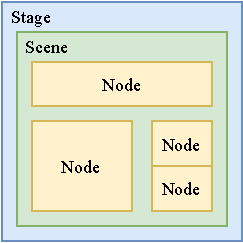
\includegraphics[width=0.35\textwidth]{fig/ainf/JavaFXStageSceneNode.pdf}
    \caption{JavaFX Stage-Scene-Node Übersicht}
    \label{fig:Stage-Scene-Node}
\end{figure}
Die die Möglichkeit zur Implementierung von Animationen, Licht/Schatten-Renderings sowie Geometrischen Objekten lässt JavaFX zu einem Vorreiter im Bereich der GUI-Entwicklung werden.
\subsubsection{Fazit}
Im Großen und Ganzen fiel aufgrund des großen Spektrums an Möglichkeiten die Wahl auf das JavaFX-Toolkit.
Obwohl JavaFX aus der Standart-Java-Bibliothek herausgeflogen ist, wird es weiterentwickelt und somit stellt ein Update kein Problem dar.
Leider erfordert es jedoch eine Einarbeitungsphase, welche aber keine Auswirkung auf den Umfang des Projekts hat.
Diese Einarbeitungsphase umfasst alle, in JavaFX verwendeten Datenformate, welche in \autoref{subsec:datenformate-in-java-fx} erklärt werden.
Außerdem muss die Verwendung von Basiselementen näher betrachtet werden, denn diese ist mit Swing-Elementen nicht zu vergleichen.
\subsection{Projektorganisation}\label{subsec:projektorganisation}
\subsubsection{Projektstruktur in Netbeans}
Eine einheitliche Formatierung und Namensgebung ist die Basis einer gelungenen Projektplanung.
Diese genannte einheitliche Formatierung führt zu einer leichteren Orientierung in fremden, aber auch in eigenen Projekten.
Um die Übersichtlichkeit eines Projektes zu verbessern, wird nach einer klar definierten Projektstruktur, welche zu Beginn des Projekts akribisch untersucht wurde, gearbeitet.
Anhand der folgenden Grafik kann die Projektstruktur dieses Projektes abgelesen werden.
\vspace{-5mm}
\begin{figure}[H]
    \begin{center}
        \begin{forest}
            for tree={
            font=\ttfamily,
            grow'=0,
            child anchor=west,
            parent anchor=south,
            anchor=west,
            calign=first,
            edge path={
            \noexpand\path [draw, \forestoption{edge}]
            (!u.south west) +(7.5pt,0) |- node[fill,inner sep=1.25pt] {} (.child anchor)\forestoption{edge label};
            },
            before typesetting nodes={
            if n=1
            {insert before={[,phantom]}}
            {}
            },
            fit=band,
            before computing xy={l=15pt},
            }
            [<project-root>
            [src
            [data
            ]
            [exception
            ]
            [gui
            ]
            [logging
            ]
            [main
            ]
            [serial
            ]
            [util
            ]
            ]
            [lib]
            [config]
            ]
        \end{forest}
    \end{center}
    \caption{Standard Projektstruktur}
    \label{porjectstructure}
\end{figure}
Der Kopf dieser Struktur beschreibt den Ordner mit dem Namen des Projekts.
Dieser wird auch \lstinline{root-directory} genannt, und ist selbst kein Package.
So spielt auch die Trennung von Sourcecode und externen Dateien eine wesentliche Rolle.
Dadurch erfolgt darunter die Aufteilung in die Ordner \lstinline{src}, \lstinline{lib}, \lstinline{config}.
\\\\
\textbf{Sourcecode}
\\
Im Ordner \lstinline{src} befindet sich der gesamte Sourcecode, wobei in diesem auch wieder eine Aufteilung in Packages erfolgt.
Diese benennen sich in diesem Fall \lstinline{data}, \lstinline{exception}, \lstinline{gui}, \lstinline{logging}, \lstinline{main}, \lstinline{serial}, und \lstinline{util}.
\\\\
\textbf{Bibliotheken}
\\
Oft werden externe Bibliotheken verwendet, welche im Ordner \lstinline{lib} gesammelt werden.
Dabei erleichtert diese Verzeichnishirachie, zu sehen in \autoref{porjectstructure} die Übersichtlichkeit aller verwendeten Bibliotheken und dessen Versionen.
Vorausgesetzt, diese werden richtig benannt.
\newpage
\textbf{Konfigurationsdateien}
\\
In unserem Fall ist es auch notwendig, einen Ordner explizit für Konfigurationsdateien vorzusehen.
Dort können Textresourcen für Sprachvarianten und Konfigurationsdateien für etwaige Aufgaben abgelegt werden.

\subsubsection{Projektstruktur für Maven und Gradle}
Das zuvor genannte Layout der Projekthirachie eignet sich gut für viele Projekte.
Jedoch zeigen sich nach und nach einige Schwachstellen an diesem System.\\
Einerseits ist das aufwendige Erstellen dieser Hirachie ein Punkt, welcher nicht unerwähnt bleiben soll.
Auch besteht ein Risiko zur Inkonstistenz bei der Namensgebung von Packages oder Bibliotheken. \\
Im Vergleich dazu, schreiben die Build-Tools Maven und Gradle eine klar definierte Projektstruktur vor.
\begin{figure}[H]
    \begin{center}
        \begin{forest}
            for tree={
            font=\ttfamily,
            grow'=0,
            child anchor=west,
            parent anchor=south,
            anchor=west,
            calign=first,
            edge path={
            \noexpand\path [draw, \forestoption{edge}]
            (!u.south west) +(7.5pt,0) |- node[fill,inner sep=1.25pt] {} (.child anchor)\forestoption{edge label};
            },
            before typesetting nodes={
            if n=1
            {insert before={[,phantom]}}
            {}
            },
            fit=band,
            before computing xy={l=15pt},
            }
            [<project-root>
            [src
            [main
            [java
            [resources]
            ]
            ]
            [test
            [java
            [resources]
            ]
            ]
            ]
            ]
        \end{forest}
    \end{center}
    \caption{Maven Projektstruktur}
\end{figure}
Diese Projektstruktur teilt sich innerhalb des \lstinline{root-directory} in 2 Bereiche auf.
Einerseits gibt es wiederum ein eigenes Package, wo sich der gesamte Sourcecode befindet.
Andererseits verfügt diese Struktur auch ein Package namens \lstinline{test}, welches ausschließlich für Tests des Codes mit dem JUnit-Framework zur Verfügung steht.\\
Trotz alledem wurde auf die althergebrachte Version der Projekterstellung gesetzt.
Grund dafür ist wiederum die fehlende Möglichkeit, eine Remote-Platform innerhalb eines Maven-Projekts zu implementieren.
Natürlich wäre eine Umstellung in einem finalen Release denkbar.
\section{Grundlagen}\label{sec:grundlagen}
\subsection{Entwurfsmuster Singelton}\label{subsec:entwurdsmuster-singelton}
\subsubsection{Beschreibung}
\footfullcite[Vgl.][]{Gamma2000}Das Entwurfsmuster namens Singelton dient dazu, die Einzigartigkeit eines Objektes sicherzustellen.
Das bedeutet, eine Instanz des Objektes ist genau einmal im Speicher vorhanden.
Zugleich bietet eine Klasse, welche nach dem Singelton-Pattern erzeugt wurde, einen globalen Zugriffspunkt über das gesamte Programm.
So ist Singelton vielseitig einsetzbar und wird in diesem Projekt häufig verwendet.
\subsubsection{Struktur}
Um nun die Einzigartigkeit sicherzustellen, sind mehrere Maßnahmen bei der Erstellung notwendig.
Realisiert wird eine Klasse, welche nach dem Singelton Design-Patter erzeugt wurde, durch einen privaten Konstruktor, denn wo keine Zugriffsberechtigung von außen herrscht, kann auch kein Objekt erstellt werden.
Dies bedeutet, dass eine Kapselung des Konstruktionsprozesses nach außen vorliegt.
Die einzige Möglichkeit, eine Instanz zu erstellen, liefert die statische Methode \lstinline{createInstance()}.
Wurde einmal eine Instanz erzeugt, also der private Konstruktor durch \lstinline{createInstance()} aufgerufen, wird diese erzeugte Instanz in einem statischen Attribut gespeichert.\\
\begin{figure}[H]
    \centering
    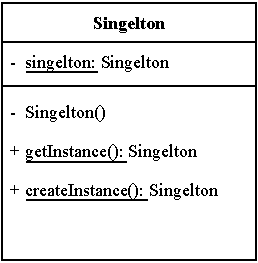
\includegraphics[width=0.35\textwidth]{fig/ainf/Singelton.pdf}
    \caption{\acs{UML}-Diagramm Singelton}
\end{figure}
Natürlich wird auch ein Zugriffspunkt auf dieses Attribut benötigt.
Implementiert wird dieser durch eine weitere statische Methode namens \lstinline{getInstance()}.
Diese Methode ist der einzige Zugriffspunkt auf die Instanz.
\subsubsection{Beispiel}
Das folgende \autoref{Singelton Code}, entnommen aus dem \textit{\autoref{subsec:konfiguration}}, zeigt wie Singelton angewendet werden kann.
% @formatter:off
\begin{lstlisting}[style=java,caption=Singelton-Codebeispiel,label=Singelton Code]
private static Config instance;

private final File configFile;
private ConfigModel configModel;

private Config(String configPath) {
    configFile = new File(configPath);
    readConfig();
}

public static Config getInstance() {
    if (instance == null) {
        throw new IllegalStateException("Instance not created yet");
    }
    return instance;
}

public static Config createInstance(String configPath) {
    if (instance != null)
        throw new IllegalStateException("Instance already created");

    instance = new Config(configPath);

    return instance;
}
\end{lstlisting}
% @formatter:on
\subsection{Verhaltensmuster Command}\label{subsec:verhaltensmuster-command}
\subsubsection{Beschreibung}
\footfullcite[Vgl.][]{Gamma2000}Ziel des Verhaltensmusters Command ist es, den jeweiligen Teilnehmer, welcher einen Befehl erzeugt, von dem Teilnehmer der für die Ausführung zuständig ist, zu entkoppeln.
Man kann auch sagen, dass der Teilnehmer, welcher den Befehlsaufruf erzeugt, nicht wissen muss, welcher Teilnehmer den Befehl empfängt oder wo bzw. wann dies geschieht.
Zugleich kann das tatsächliche Ausführen eines Befehls, aus programmatischer Sicht, in einem ganz anderen Thread geschehen, was eine elementare Rolle spielt.
Dieses Verhalten führt zu einer Vereinfachung der Ausführung von komplexeren Tätigkeiten des Programmes.
\subsubsection{Struktur}
Das Command-Pattern verfügt meist über verschieden starke Ausprägungen.
Im Kern herrscht jedoch immer dasselbe Prinzip, welches in \autoref{fig:UML-Diagramm Command} dargestellt wird.
Vor allem die Kapselung von Befehlswunsch und Ausführung steht an erster Stelle jeder jeweiligen Ausprägung.
\begin{figure}[H]
    \centering
    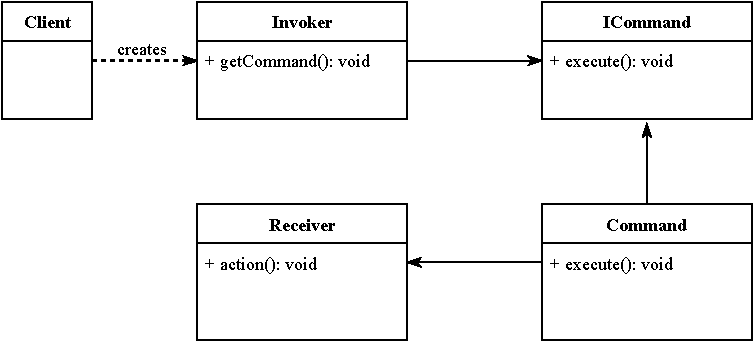
\includegraphics[width=1\textwidth]{fig/ainf/Command.pdf}
    \caption{UML-Diagramm Command}
    \label{fig:UML-Diagramm Command}
\end{figure}
\subsection{Entwurfsmuster \acs{MVC}}\label{subsec:entwurfsmuster-mvc}
\subsubsection{Beschreibung}
\footfullcite[Vgl.][]{Inden2018}Das MVC-Design Pattern, auch Model-View-Controller Design-Pattern, ist eines der weit verbreitetsten Entwurfsmuster.
Es dient zur Strukturierung von Anwendungen und teilt diese in 3 große Bereiche ab, welche strikt voneinander getrennt sind.
Mithilfe dieser Strukturierung fällt es dem Programmierer wesentlich leichter, spätere Änderungen bzw. Erweiterungen am Projekt durchzuführen, da das System nun klar definiert und strukturiert ist.
So ist es nun einfacher, parallel an dem Programm zu arbeiten, denn Ersteller von View und Ersteller des Controllers, also der Berechnungen dahinter, sind nun nicht mehr voneinander abhängig.
Jedoch muss bedacht werden, dass Änderungen am Model, direkt an die View weitergegeben werden müssen.
\newpage
\subsubsection{Struktur}
\begin{enumerate}
    \item \textbf{View}  \\
    Datenrepräsentation\\
    Organisiert alle Kontrollelemente
    \item \textbf{Controller} \\
    Stellt Verbindung zwischen View und Model her\\
    Verwaltet Benutzerinteraktion und enthält Steuerlogik
    \item \textbf{Model} \\
    Datenrepräsentation\\
    Komplett abgeschirmt von der View
\end{enumerate}
\begin{figure}[H]
    \centering
    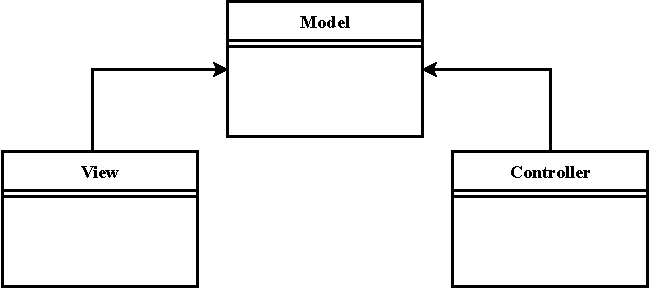
\includegraphics[width=0.8\textwidth]{fig/ainf/ModelViewController.pdf}
    \caption{UML-Diagramm MVC}
    \label{fig:UML-Diagramm MVC}
\end{figure}
\subsection{SceneBuilder}\label{subsec:scenebuilder}
\subsubsection{Beschreibung}
SceneBuilder ist ein umfangreiches GUI-Design-Tool der Firma Gluon.
Verwendet wird es bei Erstellung komplexerer Layouts, denn je komplizierter dieses wird, desto eher stößt man ohne Design-Tool an seine Grenzen.\\\\
Die Verwendung von Tools wie dieses hat mehrere Vorteile.
Einerseits verbessert sich die Übersichtlichkeit des GUI-Projekts deutlich, da es ab diesem Zeitpunkt möglich ist, den Code hinter der Oberfläche direkt grafisch darzustellen.
Andererseits kann nun nur mit wenigen Klicks, eine für den Endbenutzer ansprechende GUI gebaut werden.
Im Speziellen hat SceneBuilder weitere wichtige Vorteile, wie die direkte Verbindung mit JavaFX und dessen \lstinline{*.fxml} Dateien.
Weiters ist es möglich \acs{CSS}-Dateien sowie Internationalisierungsdateien einzubinden und diese direkt in SceneBuilder zu erweitern.
Im Wesentlichen ist SceneBuilder, gezeigt in der \autoref{fig:Tool SceneBuilder}, ein performantes Tool und eignet sich optimal für große Projekte wie dieses.
\begin{figure}[H]
    \centering
    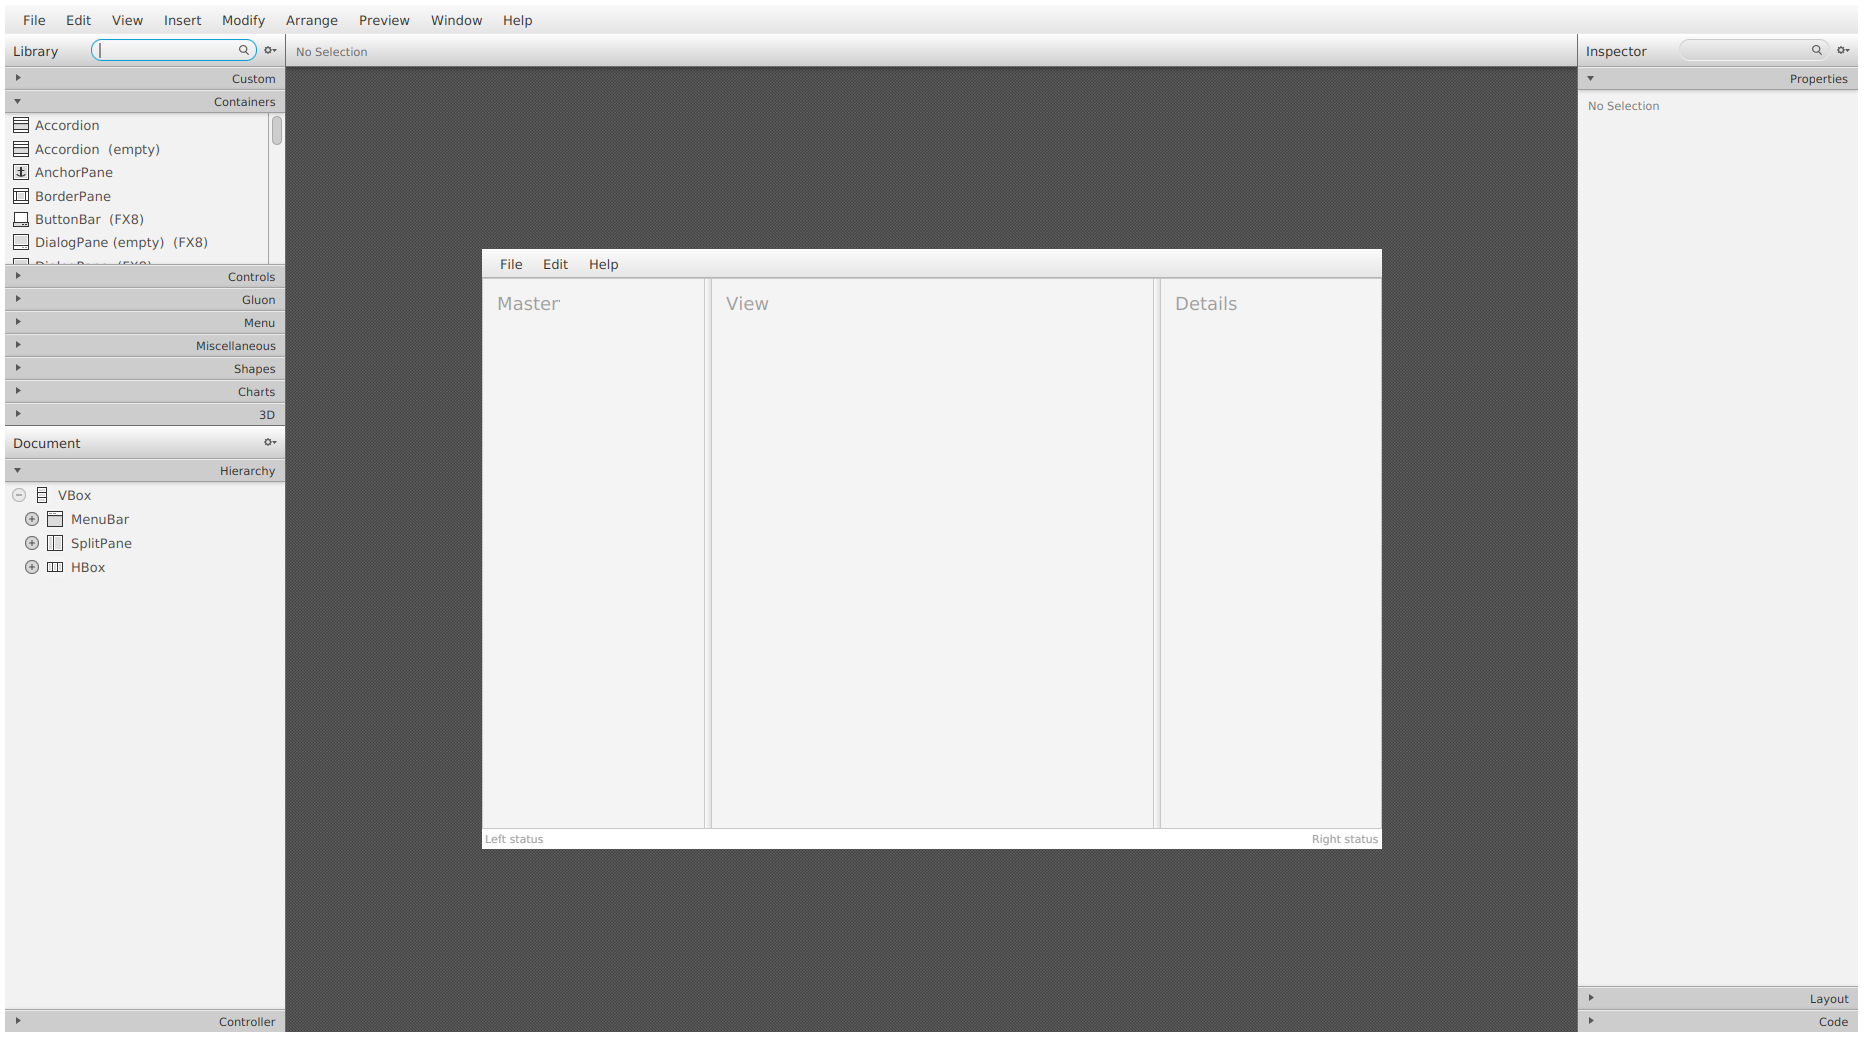
\includegraphics[width=0.8\textwidth]{fig/ainf/SceneBuilder.png}
    \caption{Tool SceneBuilder}
    \label{fig:Tool SceneBuilder}
\end{figure}
\subsubsection{Bibliothek JFoenix}
Sobald nun SceneBuilder als wichtiges Element der Erstellung ausgewählt wurde, kann ein näherer Blick auf die User-Experience geworfen werden.
Diese sogenannte User-Experience beschreibt, wie der Endbenutzer das Produkt, in diesem Fall die grafische Oberfläche empfindet.
Wird auf diesen Kernpunkt Wert gelegt, erhöht sich die Akzeptanz der Benutzer.\\\\
SceneBuilder bzw. JavaFX bieten bereits einige Grundelemente für Layouts an, diese erfüllen noch nicht die gesetzten Anforderungen.
Sie können zwar mit CSS, was im \autoref{sssec:CSS} beschrieben wird, gestaltet werden, dies ist jedoch für alle Elemente schwierig umzusetzen, da jedes Element überarbeitet werden muss.
Abhilfe schafft dabei die Material-Design-Bibliothek von JFoenix.
Diese Bibliothek ist Open-Source und implementiert, wie schon im Namen genannt, Designelemente nach dem von Google entwickelten Material-Design Vorgaben.
Das bedeutet, dass ohne viel Aufwand eine höchst ästhetische Oberfläche gebaut werden kann.
Zusätzlich kann man auch hier eigene CSS-Deklarationen vornehmen, jedoch ist vieles schon vorab definiert.\\
Anhand der folgenden \autoref{fig:Rendered Button} soll gezeigt werden, wie nun Elemente, gebaut mithilfe der JFoenix Bibliothek, aussehen.
Angewendet werden die CSS-Attribute \lstinline{-fx-border-radius: 20pt;}  \lstinline{-fx-background-radius: 20pt;} und \lstinline{-fx-background-color:grey}
\begin{figure}[H]
    \centering
    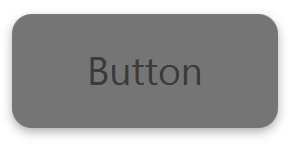
\includegraphics[width=0.4\textwidth]{fig/ainf/RenderedButton.PNG}
    \caption{Gerenderter Button}
    \label{fig:Rendered Button}
\end{figure}
\subsection{Datenformate}\label{subsec:datenformate-in-java-fx}
Im folgenden Kapitel soll auf die Datenpersistenz eingegangen werden.
Speziell in diesem Projekt werden die Datenformate \textbf{XML/FXML}, \textbf{CSS} und \textbf{\acs{JSON}} verwendet.
Ziel ist es, grundlegende Dinge zu klären und einen kurzen Überblick zu erschaffen.\\
Speziell bei JSON wird eine Bibliothek genannt, welche in diesem Projekt verwendet wurde.
\subsubsection{XML}
XML (Extensible Markup Language) ist, wie im \autoref{sssec: JavaFX} schon erwähnt, eine Sprache zur Darstellung von Daten in einem von Menschen lesbaren Format.
Damit ist sie also keine Programmiersprache.
Diese XML-Dateien sind zu vergleichen mit normalen Textdokumenten, welche mit einem gewöhnlichen Texteditor geöffnet werden können.\\
Strukturiert und bezeichnet werden in XML-Dateien die Daten mithilfe von sogenannten XML-Tags.
Diese Tags stehen in spitzen Klammern und beinhalten den Namen des Datenelementes.
Außerdem ist es notwendig, ein Start-Tag mithilfe eines sogenannten End-Tags zu schließen.
Ein Indikator für ein End-Tag ist ein \lstinline{/}.
Zwischen diesen Start- bzw.\ End-Tags befindet sich ein Datensatz.\\
Anhand der folgenden \autoref{xmlExample} soll gezeigt werden, wie XML-Dateien im Inneren aussehen.
% @formatter:off
\begin{lstlisting}[style=XML,caption=XML-Codebeispiel,label=xmlExample]
<?xml version="1.0" encoding="UTF-8"?>
    <email>
        <to>Person1</to>
        <from>Person2</from>
        <heading>Test-Header</heading>
        <body>This is a body :)</body>
    </email>
\end{lstlisting}
% @formatter:on
\subsubsection{FXML}
FXML ist ein auf XML basiertes Datenformat, welches hauptsächlich bei der Erstellung von JavaFX Anwendungen angewendet wird.
Werden FXML-Dateien zur deklarativen Beschreibung von grafischen Oberflächen genutzt, ist auch eine strikte Aufteilung nach dem \nameref{subsec:entwurfsmuster-mvc} möglich.\\
Die Struktur und Syntax von FXML-Dateien ähnelt der von XML-Dateien.
So werden auch Start- und End-Tags verwendet.
Ein wesentlicher Unterschied ist jedoch bei der Groß-/Kleinschreibung ersichtlich.
Beginnen in FXML-Dateien Elemente mit einem Großbuchstaben, werden diese als Objektdeklarationen behandelt.
Infolgedessen erkennt der FXML-Loader, welcher diese \lstinline{*.fxml} ins Programm lädt, diese Objektdeklarationen und nimmt eine dementsprechende Objektbildung vor.
Sobald diese jedoch mit einem Kleinbuchstaben beginnen, definieren sie Eigenschaften.
Eine weitere Besonderheit liegt bei dem Einbinden von Importanweisungen vor.
Diese können mithilfe des Tags \lstinline{<?import ... ?>} ausgeführt werden.
\begin{lstlisting}[style=XML,caption=FXML-Codebeispiel,label=fxmlExample]
<?xml version="1.0" encoding="UTF-8"?>
<?import javafx.scene.layout.VBox?>
<?import javafx.scene.control.Label?>

<VBox>
    <children>
    <Label text="Hello ReShuffled :)"/>
    </children>
</VBox>
\end{lstlisting}
\subsubsection{CSS}\label{sssec:CSS}
CSS ist eine Gestaltungs- und Formatierungssprache, mit welcher Gestaltungsanweisungen erstellt werden können.
Es soll aber beachtet werden, dass CSS nichts mit dem eigentlichen Inhalt der Website oder dem Programm zu tun hat, sondern rein für Design und Stilaspekte verwendet wird.\\
\footfullcite[Vgl.][]{JavaFXCSSReferenceGuide} Für unsere Anwendung bieten JavaFX Cascading Style Sheets (CSS) eine Möglichkeit, die Designziele aus dem \autoref{subsec:fronted-programmierung} umzusetzten und zu verfeinern.
Diese genannte Designsprache stellt eine Erweiterung vom standartisierten CSS mit einigen zusätzlichen Features dar.\\
Grundlegend besteht das Ziel von JavaFX CSS darin, Webprogrammierer, welche CSS bereits für Webanwendungen verwendet haben, die Möglichkeit zu geben, speziell für JavaFX zugeschnittene Themes zu bauen.
Diese Themes können auf die jeweiligen Kontrollelemente angewendet werden.\\
Eine Besonderheit von JavaFX CSS besteht im Vergleich zur normalen CSS-Sprache darin, dass alle Elemente, welche das Prefix \lstinline{-fx-...} besitzen, in direkter Verbindung mit JavaFX stehen.
Dies lässt sofort auf die Beschreibung eines JavaFX Elements schließen.
\subsubsection{JSON}\label{sssec:json}
Der Name JSON (JavaScript Object Notation) beschreibt neben XML eines der wichtigsten Datenformate zur Sicherstellung der Datenpersistenz.
Dieser Nachfolger von \acs{CSV} und INI setzt sich vor allem in der heutigen Datentechnik durch.
Grundlegend ist JSON wiederum ein textuelles Datenformat, welches kompakt und einfach lesbar ist.
Ein weiterer Grund zur Verwendung ist ebenso eine effektive Umwandlung von Daten, also Objekten, Arrays und sonstigen Variablen, in das JSON-Dateiformat.\\
All diese Merkmale sind essenziell wichtig und eröffnen ein breites Spektrum an Verwendungsmöglichkeiten.\\\\
\newpage
Die Syntax von JSON ist klar definiert und wird ebenfalls durch ein Beispiel näher visualisiert.
\begin{lstlisting}[style=json, caption=JSON-Codebeispiel,label=jsonExample]
{
    "employee": {
        "name": "tester",
        "salary": 5432,
        "children": false
    }
}
\end{lstlisting}
\textbf{Bibliothek Gson}\\
Die von Google entwickelte Bibliothek Gson spielt in diesem Projekt eine wichtige Rolle.
Bei vorhandensein von enormen Datenmengen ist es in Java zeitaufwändig, JSON-Dateien ohne zusätzliche Bibliotheken zu erstellen.\\
Eine Hilfe bietet dabei Gson.
Diese unterstützende Bibliothek hilft dem Entwickler bei der Konvertierung zwischen Java- und JSON-Objekten.
Erstellt wird eine Gson Instanz durch Erstellung des Default-Konstruktors: \lstinline[style=java]{Gson gson = new Gson()}.
Nun kann nun entweder mit der Methode \lstinline{toJson} oder mit \lstinline{fromJson} gearbeitet werden.
Diese beiden Methoden stellen die Haupteinstiegspunkte von Gson dar und werden im folgenden Teil erklärt.
\\\\
\textbf{\lstinline{toJson}}
\\
Mithilfe der Methode \lstinline[style=java]{gson.toJson()} kann direkt aus einem Objekt ein JSON-String erzeugt werden.
Dieser genannte String kann danach, je nach Belieben in eine Datei geschrieben oder versendet werden.
\\\\
\textbf{\lstinline{fromJson}}
\\
Außerdem kann der gesamte Prozess mithilfe des Methodenaufrufs \lstinline[style=java]{gson.fromJson()} umgekehrt werden.
Hierbei wird aus einem JSON-String ein Objekt erzeugt.
\newpage
\section{Backend-Programmierung}\label{sec:backend-programmierung}
\subsection{Kommunikation}\label{subsec:kommunikation}
\subsubsection{Konzept}
Um erfolgreich Daten zwischen dem Raspberry Pi 3B+ und der Platine, welche die Ansteuerung sämtlicher Komponenten übernimmt, zu übertragen, wird ein Kommunikationsprotokoll benötigt.
Dieses Protokoll stellt im engsten Sinne eine Vereinbarung dar, wie die Datenübertragung zwischen zwei oder mehreren Parteien abläuft.
Anforderungen an dieses Protokoll sollen sein:
\begin{enumerate}
    \item Einfache Implementierung in den Zielsystemen
    \item Erweiterbarkeit des Protokolls mit geringem Arbeitsaufwand
    \item Hohe Sicherheit gegenüber Übertragungsfehler
    \item Schnelle Fehlererkennung sowie Fehlerbehebung
\end{enumerate}
Neben standardisierten Protokollen wie Modbus, Feldbus oder CAN-Bus gibt es die Möglichkeit, selbst ein sogenanntes propretäres Übertragungsprotokoll zu definieren.
Dies ist in unserem Fall möglich, um alle Anforderungen abzudecken.
Basierend auf dem Master-Slave Prinzip, wobei der Raspberry Pi den Master und die Ansteuerplatine den Slave darstellt, soll ein an Modbus-\acs{ASCII} angelehntes Protokoll umgesetzt werden.\\
Zusätzlich soll, um eine virtuelle Testumgebung zur Kommunikation zu schaffen, ein Simulator ausprogrammiert werden, welcher beim Start, auf Softwarebebene den Platz des Slaves bzw. der Ansteuerplatine einnimmt.
Der Startvorgang des Simulators soll mit einer einfachen Modifizierung der Konfigurationsdatei vonstattengehen.
Die folgende Grafik soll schematisch die Geräteauswahl darstellen.
\begin{figure}[H]
    \centering
    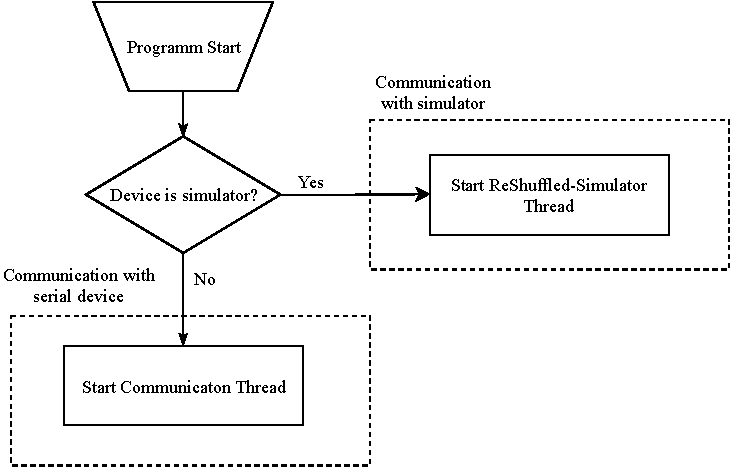
\includegraphics[width=0.7\textwidth]{fig/ainf/DeviceSelection}
    \caption{Schematische Darstellung der Geräteauswahl}
    \label{deviceSelection}
\end{figure}
\subsubsection{Übertragungsprotokoll} \label{sssec:uebertragungsprotokoll}
\begin{table}[H]
    \centering
\resizebox{\textwidth}{!}{%
    \begin{tabular}{|
    >{\columncolor[HTML]{FFFFFF}}l |
    >{\columncolor[HTML]{FFFFFF}}l |
    >{\columncolor[HTML]{FFFFFF}}l |
    >{\columncolor[HTML]{FFFFFF}}l |
    >{\columncolor[HTML]{FFFFFF}}l |}
        \hline
        \textbf{Doppelpunkt :} & \textbf{Daten (ASCII)} & \textbf{Trennzeichen \#} & \textbf{CRC32-Prüfsumme} & \textbf{Line Feed Character \textbackslash{}n} \\ \hline
        8-Bit & 16-Bit & 8-Bit & 32-Bit & 8-Bit                                \\ \hline
    \end{tabular}
}
    \caption{Visualisierung des Datenakets}
\end{table}
Das verbindungslose Protokoll basiert, wie in der Konzeptbeschreibung bereits erwähnt, auf dem Master-Slave Prinzip.
Die Datenübertragung erfolgt rein textuell, wobei nur Großbuchstaben verwendet werden dürfen.\\\\
Wie aus der oben dargestellten Tabelle zu entnehmen, ist der Aufbau eines Frames klar definiert.
Der eindeutige Start des Datenpakets, welcher mit einem Doppelpunkt (:) eingeleitet wird, sowie das ebenfalls eindeutige Ende, umgesetzt mit einem Line Feed Character (\verb!\n!), bringt eindeutige Vorteile mit sich.
Im Gegensatz zu anderen Protokollen wie z.B. Modbus-RTU, muss hier nicht auf das Ende des Pakets "gewartet" werden.
Dies führt zu einer erschwerten Umsetzung und ist für uns nicht zielführend.\\\\
Gefolgt von dem Startzeichen folgen nun die Daten.
Diese beinhalten eindeutig definierte Zeichenfolgen, welche verwendet werden, um verschiedenste Zustände der Ansteuerplatine auszuführen.
Nachfolgend schlie"st das Trennzeichen (\verb!#!) diese Daten ab.\\\\
Um nun die Integrität, also die Korrektheit der Daten, bei einer Übertragung zu überprüfen, wird im danach eine Prüfsumme übertragen.
Ziel dieser ist es, anhand der Nutzdaten(16-Bit Request-String) einen Wert zu bilden, welcher danach vom Sender im Frame als hexadezimalen String gespeichert bzw. übertragen wird.
Der Empfänger berechnet nun mit demselben Verfahren die Prüfsumme aus den empfangenen Daten und vergleicht diese mit der übertragenen Prüfsumme des Senders.
Sind beide Prüfsummen identisch, war die Übertragung erfolgreich und die Daten sind mit großer Wahrscheinlichkeit korrekt.
Stimmen diese nicht überein, liegt ein Fehler vor.
Die wichtigsten Arten von Übertragungsfehlern sind:
\begin{enumerate}
    \item Einzelbitfehler (1 Bit verändert)
    \item Burstfehler (ganze Folge von Bits verändert)
\end{enumerate}
Neben einfachen Verfahren wie z.B. dem Paritätsbit-Verfahren gibt es auch effizientere Vorgehensweisen.
Die zyklische Redundanzprüfung, auch \acs{CRC} genannt, ist eines davon.
Sie ist relativ einfach zu realisieren und dennoch wirkungsvoll.
Wichtig beim CRC-Verfahren ist, dass beide Teilnehmer, also Sender und Empfänger, dasselbe Schema zur Berechnung bzw. Verarbeitung der Prüfsumme verwenden.
Hierbei spielt der Grad des Generator-Polynoms sowie die mögliche Invertierung der Bits vor dem Sendevorgang eine wesentliche Rolle.
Der Grad des Generator-Polynoms beträgt in unserem Fall 32 (CRC-32) und die Prüfsumme wird nicht invertiert.\\\\
Zusätzlich soll definiert werden, welche Ma"snahmen getroffen werden, wenn kein Response ankommt.
Ist dies der Fall, wird je nach Wert eines Eintrags in der Konfigurationsdatei, ein weiterer Request mit demselben Inhalt gesendet.
Kommt nun wiederum kein Response an, soll eine spezifische Exception geworfen werden.\\
Wichtig ist auch die Definition des Fehlerhandlings.
So muss, wenn ein Response mit dem Fehler-Prefix (E) in den Nutzdaten ankommt, eine Ma"snahme getroffen werden.
Diese soll in Form eines Log-Eintrags sowie einer Exception vonstattengehen, da es sich hierbei um gravierende Fehler beim Verarbeiten auf dem Endgerät handeln muss.
\subsubsection{Request- und Responsebeispiele}
Aufgrund eines wohldurchdachten Systems bei der Request-Definition, ist es nun möglich, den Pool an verschiedenen Requests explizit zu minimieren.
Dies bezieht sich auf den Vorgang der automatischen Kartenverteilung an jeden einzelnen Spieler, was mithilfe des Requests \textit{Deal} und \textit{AutoDeal} umgesetzt wird.\\
Neben diesen genannten Requests, welche sich rein auf den Ablauf eines Kartenspiels konzentrieren, verfügt der Pool an Requests, welche allgemein zur Funktionalität der Maschine beitragen.
Der Request \textit{Shutdown} führt lediglich zu einem Herunterfahren der Maschine.
Darüber hinaus trägt der Request \textit{Init}, welcher nach jedem Startvorgang ausgeführt wird, zur allgemeinen Funktion der Maschine bei.
Dieser hat den Sinn und Zweck, die Maschine in einen Initialisierungszustand zu versetzten.
\begin{table}[H]
    \centering
    \resizebox{\textwidth}{!}{%
        \begin{tabular}{|l|l|l|c|}
            \hline
            \rowcolor[HTML]{FFFFFF}
            \textbf{Request} & \textbf{Request-String {[}Rx{]}} & \textbf{Aktion} & \multicolumn{1}{l|}{\cellcolor[HTML]{FFFFFF}\textbf{Response-String {[}Tx{]}}} \\ \hline
Init     & IN                                          & Initialisierungs-Zustand     & \multicolumn{1}{l|}{OK oder E\textless{}Code\textgreater{}} \\ \hline
Shutdown & XX                                          & Herunterfahren der Maschine  & \multicolumn{1}{l|}{OK oder E\textless{}Code\textgreater{}} \\ \hline
Shuffle  & SH                                          & Mischen von Karten           & \multicolumn{1}{l|}{OK oder E\textless{}Code\textgreater{}} \\ \hline
Deal     & D\textless{}Anzahl der Karten\textgreater{} & Kartenausgabe je nach Anzahl & \multicolumn{1}{l|}{OK oder E\textless{}Code\textgreater{}} \\ \hline
AutoDeal & A\textless{}Anzahl der Karten\textgreater{} & Automatische Kartenausgabe   & \multicolumn{1}{l|}{OK oder E\textless{}Code\textgreater{}} \\ \hline
\end{tabular}%
}
\caption{Request-Response Pool}
\end{table}
Folgend wird anhand von tabellarisch aufgelisteten Beispielen gezeigt, wie ein Request mit dem jeweiligen Response zusammenhängt.
Jeder Request sowie Response basiert auf der Protokolldefinition aus dem \autoref{sssec:uebertragungsprotokoll}.
\begin{table}[H]
\centering
\begin{tabular}{|l|l|l|}
\hline
{\color[HTML]{333333} \textbf{Request}} & {\color[HTML]{333333} \textbf{Example Request Frame}} & {\color[HTML]{333333} \textbf{Example Response Frame}} \\ \hline
{\color[HTML]{333333} Init}             & {\color[HTML]{333333} :IN\#F1068A24\textbackslash{}n} & {\color[HTML]{333333} :E1\#9D09A985\textbackslash{}n}  \\ \hline
{\color[HTML]{333333} Shutdown}         & {\color[HTML]{333333} :XX\#560B1C65\textbackslash{}n} & {\color[HTML]{333333} :OK\#D736D92D\textbackslash{}n}  \\ \hline
{\color[HTML]{333333} Shuffle}          & {\color[HTML]{333333} :SH\#A848D5CA\textbackslash{}n} & {\color[HTML]{333333} :E1\#9D09A985\textbackslash{}n}  \\ \hline
{\color[HTML]{333333} Deal}             & {\color[HTML]{333333} :D1\#841298C4\textbackslash{}n} & {\color[HTML]{333333} :OK\#D736D92D\textbackslash{}n}  \\ \hline
{\color[HTML]{333333} \acs{AutoDeal}}         & {\color[HTML]{333333} :A5\#FE08A898\textbackslash{}n} & {\color[HTML]{333333} :E1\#9D09A985\textbackslash{}n}  \\ \hline
\end{tabular}
\caption{Request-Response Beispiele}
\end{table}
\subsubsection{Umsetzung-Datenaustausch}
Zuallererst soll der Ablauf der Kommunikation zwischen dem Programm und dem Endgeräts, welches über die serielle Schnittstelle verbunden ist, betrachtet werden.
Im ersten Schritt wird auf die Erstellung jedes einzelnen Request eingegangen.\\
Um die Einbindung von Requests elegant und objektorientiert umzusetzen, stellt die abstrakte Klasse \lstinline[style=java]{Request} die Elternklasse jedes einzelnen Request dar.
Dies bedeutet im engsten Sinne, dass jeder einzelne Request eine Ableitung dieser Klasse ist.
Dargestellt wird dies auch durch das generierte UML-Diagramm in \autoref{umlReq}.
\begin{figure}[H]
\centering
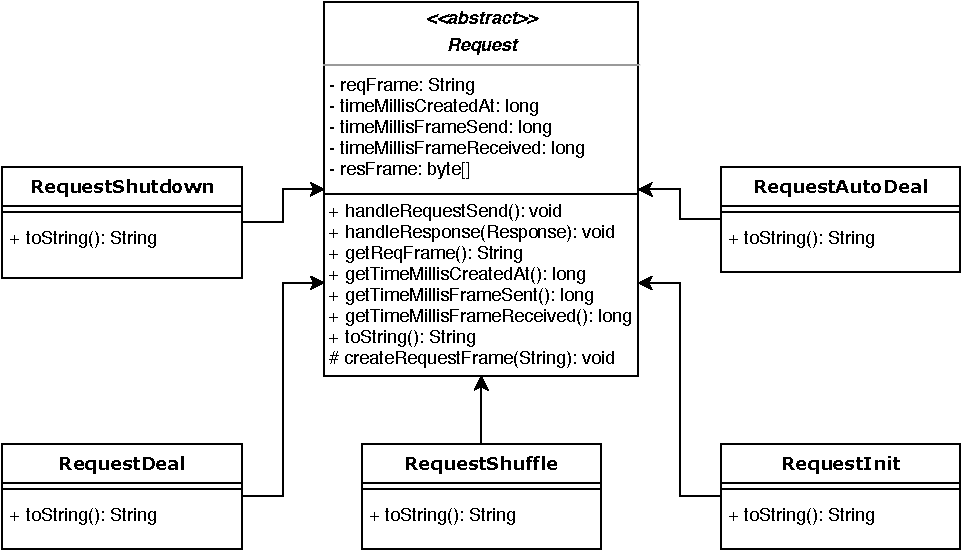
\includegraphics[width=1\textwidth]{fig/ainf/AbstractRequestUML.pdf}
\caption{UML-Diagramm Request-Baum}
\label{umlReq}
\end{figure}
Bevor nun auf jeden einzelnen Request eingegangen wird, soll nun die abstrakte Klasse \lstinline[style=java]{Request} betrachtet werden.
Diese Klasse implementiert die Methoden \lstinline[style=java]{createRequestFrame()},\\ \lstinline[style=java]{handleRequestSent()} und \lstinline[style=java]{handleResponse()}.\\\\
Wie der Name der Methoden schon ahnen lässt, ist \lstinline[style=java]{createRequestFrame()} für die Erstellung jedes Request zuständig.
Diese Methode besitzt den Zugriffsmodifizierer \lstinline[style=java]{protected} und kann somit von den abstammenden Requests aufgerufen werden.
% @formatter:off
\begin{lstlisting}[style=java,caption=Methode createRequestFrame(),label=Gesamte Methode createRequestFrame()]
private static java.util.zip.CRC32 CRC32 = new java.util.zip.CRC32();
private String reqFrame;

protected void createRequestFrame(String content) {
    if (content == null || content.isEmpty()) {
        throw new IllegalArgumentException();
    }
    CRC32.reset();
    CRC32.update(content.getBytes());
    final String crc32 = String.format("%08X", CRC32.getValue());
    final StringBuilder sb = new StringBuilder(128);
    sb.append(':').append(content).append('#').append(crc32).append('\n');
    reqFrame = sb.toString();
}
\end{lstlisting}
% @formatter:on
Sobald die Methode von einem abstammenden Request aufgerufen wird und der Content, also der Request-String, übergeben wird, überprüft diese Methode den übergebenen Content.
Sollte dieser leer sein wird eine \lstinline[style=java]{IllegalArgumentException} geworfen und die Erstellung des Requests wird somit abgebrochen.
Ist jedoch ein Content vorhanden, wird mithilfe der Bibliothek \lstinline{java.util.zip.CRC32} eine CRC-32 Prüfsumme erzeugt und in ein hexadezimales Format geparst.
Letztendlich wird danach der Request-String mithilfe eines \lstinline{StringBuilders} zusammengebaut.
Das für die Datenspeicherung im Objekt zuständige Attribut benennt sich \lstinline[style=java]{private String reqFrame} und speichert dessen Daten in einem String.\\\\
Weiters verfügt die Klasse die Methode \lstinline[style=java]{handleRequestSent()}, welche ausschließlich die Aufgabe hat, den definierten Zeitstempel \lstinline[style=java]{timeMillisFrameSent} zu setzten.
Dieser genannte Zeitstempel ist im nachhinein für das Timeout-Handling von Responses wichtig.\\
Sobald nun ein Response ankommt, kommt die Methode \lstinline[style=java]{handleResponse()} ins Spiel.
Aufgabe dieser ist es, das ankommende Response-Objekt, welches im unteren Abschnitt beschrieben wird, in dessen elementaren Daten zu zerlegen.
%\lstinputlisting[firstline=35, lastline=42, style=java,caption=Teilabschnitt Methode handleResponse(),label=handleResponse() Teilabschnitt]{src/serial/request/Request.java}
% @formatter:off
\begin{lstlisting}[style=java,caption=Teilabschnitt Methode handleResponse(),label=handleResponse() Teilabschnitt]
public void handleResponse(Response res) throws SerialException {
    timeMillisFrameReceived = res.getTimeMillisCreatedAt();
    byte[] receivedContentCRC = new byte[2];
    String receivedCRC = "", receivedContent = "";
    CRC32.reset();
    resFrame = res.getResFrame();
    LOG.fine("Received response " + Arrays.toString(resFrame));
    ...
}
\end{lstlisting}
% @formatter:on
Zugleich soll in dieser Methode überprüft werden, ob der Content des Frames Fehler aufweist.
Dies geschieht wieder mithilfe der in Java implementierten Bibliothek \lstinline{CRC32} und soll nicht näher beleuchtet werden.
Nun wird anhand des zurückkommenden Response-Strings analysiert, wie sich der Request im Zielsystem verhalten hat.
Wie im Protokoll definiert, kann nun entweder ein \lstinline[style=java]{OK} oder ein Errorcode mit dem Prefix \lstinline[style=java]{E} zurückkommen.
Der Pool an Codes kann jedoch nur ein Volumen von neun annehmen, da ansonsten der Frame zu groß wäre.
Umgesetzt wird die Analyse mithilfe einer switch-case-Verzweigung.
%\lstinputlisting[firstline=61, lastline=86, style=java,caption=fdsa,label=handleResponse() Teilabschnitt]{src/serial/request/Request.java}
Jeder einzelne Error steht für eine spezielle Fehlerquelle bei der Ausführung.\\\\
Zusätzlich wird in der Klasse \lstinline[style=java]{Request} die \lstinline[style=java]{toString()} Methode überlagert.
Dadurch kann das Request Objekt nun optimal in einen String umgewandelt werden.
Nun betrachten wir die spezifischen Requests, welche in \autoref{umlReq} zu sehen sind.\\
Im Prinzip ist der Aufbau jeder Request-Klasse ähnlich.
Aufgerufen wird der Konstruktor, welcher die Methode \lstinline[style=java]{createRequestFrame()} ausführt.
Als Parameter erhält diese Methode den vom Protokoll festgelegten Content.
Anhand eines Beispiels soll der Request \textit{Shuffle} gezeigt werden.
\lstinputlisting[firstline=8, lastline=12, style=java,caption=Konstruktor RequestShuffle(),label=toString() Methode]{src/serial/request/RequestShuffle.java}
\textbf{Fazit}\\
Somit erhält man nach Erstellung eines Objekts vom gewählten Request-Typ ein vollwertiges Objekt, mit dem gearbeitet werden kann.
Im folgenden Abschnitt wird nun gezeigt, wie ein Request versendet werden kann.\\\\
Die gesamte Kommunikation wird umgesetzt durch die Klasse \lstinline[style=java]{Communication}.
Diese kann verglichen werden mit einem Service, welcher sich um das Senden und Empfangen von Daten kümmert.
Die vom Design-Pattern Singelton abgeleitete Klasse, stellt zwei Threads bereit, wobei einer davon für den Sendungs- und einer für den Empfangsvorgang zuständig ist.
Beide werden im privaten Konstruktor der Klasse erstellt und gestartet.
Somit ist ab diesem Zeitpunkt die Verfügbarkeit zur Kommunikation gegeben.\\\\
\textbf{Der CommunicationSendThread}\\
Nun besteht jedoch das Problem, dass diese zwei Threads untereinander abgestimmt werden müssen.
Ein wichtiges Beispiel zeigt hierbei das Producer-Consumer-Problem, welches in der \autoref{ProducerConsumer} dargestellt wird.
\begin{figure}[H]
\centering
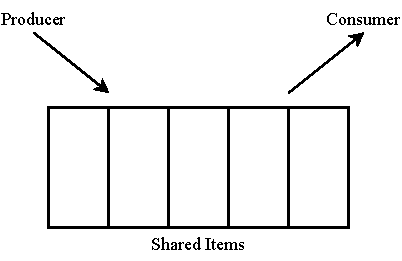
\includegraphics[width=0.45\textwidth]{fig/ainf/ProducerConsumer.pdf}
\caption{Kommunikation Producer-Consumer}
\label{ProducerConsumer}
\end{figure}
\newpage
Dieses Problem bezieht sich auf die gemeinsame Verwendung von Items, da hier Überschneidungen entstehen.
In diesem Fall stellt die sogenannte \lstinline[style=java]{toSentList}, welche als \lstinline[style=java]{LinkedList} vom Typ \lstinline[style=java]{Request} implementiert wurde, die Items dar.
Einerseits müssen hier Requests zur Liste hinzugefügt und andererseits entnommen werden.\\
Um nun die Thread-Sicherheit zu gewährleisten und Deadlocks zu vermeiden, wurde in kritischen Abschnitten vom Schlüsselwort \lstinline[style=java]{synchronized()} gebrauch gemacht.
Wie schon im oberen Teil beschrieben, bietet die sogenannte \lstinline[style=java]{toSentList} eine gemeinsame Ablage von Requests.
Bei jedem Zugriff wird nun also mit \lstinline[style=java]{synchronized(toSentList)} gearbeitet.
Mithilfe der Methoden \lstinline[style=java]{wait()} und \lstinline[style=java]{notify()} wurde also eine Möglichkeit geschaffen, um Busy-Waiting zu vermeiden.
Hier wartet bzw. schläft der Thread, bis er von außen aktiviert, also aufgeweckt wird.
Zu sehen ist dies im \autoref{commThreadSync}.
% @formatter:off
\begin{lstlisting}[style=java,caption=Teilabschnitt CommunicationSendThread,label=commThreadSync]
...
try {
    mainLoop:
    while (!Thread.currentThread().isInterrupted()) {
        synchronized (toSentList) {
            LOG.fine("Thread waiting for items ...");
            toSentList.wait();

            if (!toSentList.isEmpty()) {
            ....
            }
        }
    }
}
catch (Exception ex) {
    LOG.warning(ex, Thread.currentThread().getName() + " exception");
}
finally {
    LOG.info(Thread.currentThread().getName() + " ended");
}
...
\end{lstlisting}
% @formatter:on
Hinzugefügt kann ein Item über die Methode \lstinline[style=java]{public void sendRequestExecutor (Request req)} werden.
Diese Methode, welche nach dem Command-Verhaltensmuster (\autoref{subsec:verhaltensmuster-command}) gestaltet wurde, fügt lediglich ein Element zur Liste hinzu und weckt den Thread mit \lstinline[style=java]{notifyAll()}.
%\lstinputlisting[firstline=61, lastline=67, style=java,caption=Methode sendRequestExecutor(),label=toString() Methode]{src/serial/Communication.java}
% @formatter:off
\begin{lstlisting}[style=java,caption=Methode sendRequestExecutor(),label=sendRequestExecutor()]
public void sendRequestExecutor(Request req) {
    synchronized (toSentList) {
        toSentList.add(req);
        toSentList.notifyAll();
    }
}
\end{lstlisting}
% @formatter:on
Befindet sich nun etwas in der \lstinline[style=java]{toSentList}, beginnt der Thread zu arbeiten.
Ein Loop zur Sendung eines Request kann einfach anhand des \autoref{commThreadSend} erklärt werden.
% @formatter:off
\begin{lstlisting}[style=java,caption=Teilabschnitt CommunicationSendThread,label=commThreadSend]
...
if (!toSentList.isEmpty()) {
    pendingRequest = toSentList.removeFirst();
    LOG.fine("sending request " + pendingRequest.getMreqFrame());
    serial.writeString(pendingRequest.getMreqFrame());
    pendingRequest.handleRequestSent();
}
...
\end{lstlisting}
% @formatter:on
Vorerst wird der wartende Request in dem Attribut \lstinline[style=java]{Request pendingRequest} gespeichert und von der Liste gelöscht.
Danach kann dieser über die serielle Schnittstelle versendet werden.
Dies erfolgt mithilfe der Hilfsmethode \lstinline[style=java]{serial.writeString()}, welche im \autoref{sssec:deviceSelection} beschrieben wurde.\\\\
Nun soll auf den ankommenden Response gewartet werden.
So wird auch hier eine \lstinline[style=java]{LinkedList} implementiert.
Diese besteht jedoch nicht aus Request-Objekten, sondern aus sogenannten Response-Objekten.
In jedem einzelnen Objekt vom Typ \lstinline[style=java]{Response} befindet sich der Frame, gespeichert in dem Attribut \lstinline[style=java]{byte [] resFrame}, und ein Zeitstempel namens \lstinline[style=java]{long timeMillisCreatedAt}.\\\\
Wird nun vom CommunicationReceiveThread, welcher später beschrieben wird, ein Request empfangen und zur \lstinline[style=java]{responseList} hinzugefügt, entfernen die folgenden Zeilen Code den Request von der Liste und speichern diesen.
Befinden sich jedoch mehrere Elemente in der Liste, ist dies ein Indiz für einen Fehler.
Sollte dieser Fall auftreten, wird dies mithilfe einer Warnung in der Log-Datei dargestellt.
Außerdem wird nur immer der erste Request verwendet und sämtliche Requests, welche sich danach in der Liste befinden, gelöscht.
% @formatter:off
\begin{lstlisting}[style=java,caption=Teilabschnitt CommunicationSendThread,label=commThreadSend]
...
res = responseList.removeFirst();
if (!responseList.isEmpty()) {
    LOG.warning("response list should be empty, but " + responseList.size() + " items in list");
    responseList.clear();
}
...
\end{lstlisting}
% @formatter:on
Mithilfe des Methodenaufrufs \lstinline[style=java]{pendingRequest.handleResponse(res)} wird nun, wie oben beschrieben, der Response weiter verarbeitet.\\\\
Sollte jedoch kein Response ankommen, versucht das Programm, sofern in der Konfigurationsdatei ein zweiter Versuch erlaubt ist, den selben Request nochmals zu senden.
Ist dies nicht der Fall, wird eine \lstinline[style=java]{SerialException} geworfen.
% @formatter:off
\begin{lstlisting}[style=java,caption=Teilabschnitt CommunicationSendThread,label=commThreadSend]
...
if (responseList.isEmpty()) {
    if (Config.getInstance().getConfigSerial().isSecondTryAllowed()) {
        sendRequestExecutor(pendingRequest); //send second response
        continue mainLoop;
    }
    throw new SerialException("request timeout, missing response");
}
...
\end{lstlisting}
% @formatter:on
Somit wäre ein Kommunikations-Loop abgeschlossen und der CommunicationSendThread wartet wieder auf ankommende Requests des Programms.\\\\
\textbf{Der CommunicationReceiveThread:}\\
Nun sollte jedoch das Empfangen eines Response näher beschrieben werden.
Dieser sogenannte CommunicationReceiveThread holt sich vorerst den InputStream und liest danach die Zeichen ein.
Ist das ankommende Zeichen das Startzeichen(\lstinline[style=java]{:}), beginnt er, die folgenden Zeichen einschließlich des \lstinline[style=java]{:} in einen Buffer zu speichern.
Sollte jedoch ein unerwartetes Zeichen ankommen, was auf einen Übertragungsfehler hinweist, wird ein Eintrag in die Log-Datei erstellt, welcher den Fehler veranschaulicht.
% @formatter:off
\begin{lstlisting}[style=java,caption=Teilabschnitt CommunicationReceiveThread,label=commThreadSend]
...
while (!Thread.currentThread().isInterrupted()) {
    int b = is.read();
    if (b >= 0 && b < 255) {
        if (bufferIndex == 0) {
            if (b == ':') {
                buffer[bufferIndex++] = (byte) b;
            }
            else {
                LOG.warning("receiving unexpected byte
                    (':' expected, get " + b);
            }
        }
...
\end{lstlisting}
% @formatter:on
Werden die ankommenden Daten nun als vollwertigen Request erkannt, fügt der CommunicationReceiveThread diesen zur oben genannten \lstinline[style=java]{responseList} hinzu und weckt den CommunicationSendThread, welcher diesen, wie oben beschrieben, weiterverarbeitet.
\newpage
% @formatter:off
\begin{lstlisting}[style=java,caption=Teilabschnitt CommunicationReceiveThread,label=commThreadSend]
...
else if (bufferIndex < buffer.length) {
    buffer[bufferIndex++] = (byte) b;
    if (b == '\n') {
        synchronized (responseList) {
            byte[] resBuffer = Arrays.copyOf(buffer, bufferIndex);
            bufferIndex = 0;
            responseList.add(new Response(resBuffer));
            responseList.notifyAll();
        }
    }
}
else {
    LOG.warning("receiving byte " + b + " cannot be stored (receive buffer overflow)");
}
...
\end{lstlisting}
% @formatter:on
\subsubsection{Geräteauswahl} \label{sssec:deviceSelection}
%Nachdem nun ausführlich über den Serial-Simulator gesprochen wurde, wird nun im Folgenden die Geräteauswahl beschrieben.\\
Wie in der \autoref{deviceSelection} gezeigt, erfolgt die Auswahl des Gerätes, mit welchem kommuniziert wird, bei jedem Startvorgang.
Zuständig für diese Referenzierung des Endgeräts ist die Klasse \lstinline[style=java]{Serial}, welche alle dafür benötigten Methoden bereitstellt.
Designt wurde diese Klasse nach dem Singelton-Entwurfsmuster was in der \autoref{umlSerial} ersichtlich ist.
\begin{figure}[H]
\centering
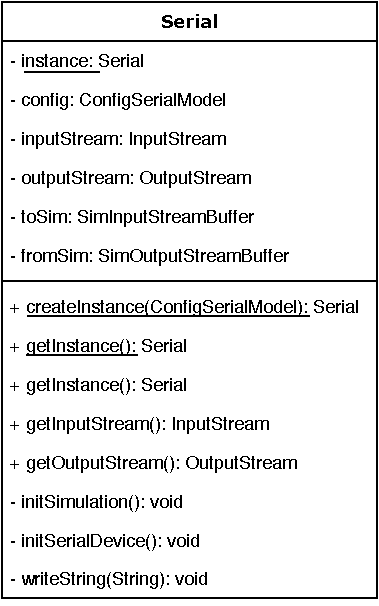
\includegraphics[width=0.35\textwidth]{fig/ainf/SerialUML.pdf}
\caption{UML-Diagramm Serial}
\label{umlSerial}
\end{figure}
Im ersten Schritt erfolgt die Untersuchung der Konfigurationsdatei.
Ist hier der Eintrag \lstinline[style=json]{"device": "sim"} vorhanden, wird der Simulator gestartet und alle notwendigen Konfigurationen werden vorgenommen.
Sollte jedoch etwas anderes eingetragen sein, wird versucht mit dem seriellen Gerät zu kommunizieren.
Ist dies der Fall, muss auch die serielle Schnittstelle vor der Verwendung konfiguriert werden.\\
All diese Aufgaben übernimmt die vom Design-Pattern-Singelton abgeleitete Klasse \lstinline[style=java]{Serial} und wird im folgenden Abschnitt beschrieben.\\\\
Wird im ersten Schritt eine Instanz der Klasse Serial mithilfe der Methode \lstinline[style=java]{createInstance()} erstellt, wird der private Konstruktor aufgerufen.
Dieser hat 2 wesentliche Aufgaben.\\
Einerseits soll er sicherstellen, dass sich alle Parameter der seriellen Schnittstelle in der Konfigurationsdatei befinden.
Umgesetzt wird dies mithilfe der Abfrage \lstinline[style=java]{if (config.isDisabled())}.
Diese Parameter werden im Folgenden aufgelistet.
% @formatter:off
\begin{lstlisting}[style=json,caption=Teilabschnitt Konfigurationsdatei,label=jsonSerial]
"serial": {
    "disabled": false,
        "device": "sim",
        "baudrate": 57600,
        "timeoutMillis": 1000,
        "secondTryAllowed": false,
        "responseByteLength": 32
},
\end{lstlisting}
% @formatter:on
Andererseits soll die Geräteauswahl mithilfe eines Abgleichs des Gerätenamens erfolgen.
Wird die Zeichenkette \lstinline[style=json]{"sim"} mithilfe der Abfrage \lstinline[style=java]{if (config.getDevice().equals("sim"))} erkannt, wird die Methode \lstinline[style=java]{initSimulation()}, ansonsten \lstinline[style=java]{initSerialDevice()} ausgeführt.
In diesen beiden Methoden werden sowohl die serielle Schnittstelle, als auch der Simulator konfiguriert.
Nun soll anhand der Listings näher auf den Code der beiden Methoden eingegangen werden.
% @formatter:off
\begin{lstlisting}[style=java,caption=Konstruktor Serial(),label=serialInit]
private Serial(ConfigSerialModel config) throws SerialException, IOException {
    this.config = config;

    if (config.isDisabled()) {
        return;
    }
    if (config.getDevice().equals("sim")) {
        initSimulation();
    } else {
        initSerialDevice();
    }
}
\end{lstlisting}
% @formatter:on
\textbf{\lstinline{initSimulation()}}
\\
Vorerst soll angenommen werden, dass als Gerät der Simulator ausgewählt wurde.
Ist dies der Fall, wird innerhalb der Methode \lstinline{initSimulation()} eine Möglichkeit zur Kommunikation mit dem Simulator geschaffen.
Realisiert wird diese Verbindung, wie im anschließenden \autoref{sssec:serialSim} beschrieben, mithilfe von Input- und OutputStreams.
Also werden diese zu Beginn definiert.\\
Um nun den Serial-Simulator zu starten ist lediglich eine Erstellung des ReshuffledMainboardSimulator-Objekts notwendig.
Dieser erhält einen Input- und OutputStream mit welchen er die Kommunikation durchführen kann.\\\\
So ist nun die volle Funktionalität des Simulators gegeben und es kann ohne echte Peripherie gearbeitet werden.
%\lstinputlisting[firstline=69, lastline=87, style=java,caption=Methode initSimulation(),label=fdsafdsa]{src/serial/Serial.java}
% @formatter:off
\begin{lstlisting}[style=java,caption=Methode initSimulation(),label=fdsafdsafds]
private void initSimulation() throws IOException {
    toSim = new SimInputStreamBuffer();
    fromSim = new SimOutputStreamBuffer();
    inputStream = new InputStream() {
        @Override
        public int read() throws IOException {
            return fromSim.read();
        }
        @Override
        public int available() throws IOException {
            return fromSim.available();
        }
    };
    outputStream = new SerialSimOutputStream();
    new ReshuffledMainboardSimulator(toSim, fromSim);
    LOG.info("serial simulation activated");
}
\end{lstlisting}
% @formatter:on
\textbf{\lstinline{initSerialDevice()}}
\\
Wird nun angenommen, dass es sich bei dem Konfigurationseintrag nicht um die Zeichenkette \lstinline[style=json]{"sim"} handelt, springt das Programm in die Methode \lstinline{initSerialDevice()}.
Erfolgt nun das Einlesen der im \autoref{jsonSerial} gezeigten Parameter, wird der Port zum Endgerät geöffnet.\\
Verwendet wurde hierbei die Open-Source-Bibliothek \acs{jSSC} (Java Simple Serial Connector).
Erstellt wird eine Instanz des \lstinline[style=java]{jssc.SerialPort} mithilfe einer Objekterzeugung.
Diese fordert als Parameter den Namen des Ports.
Nun kann mithilfe der Methode \lstinline{openPort()} der Port geöffnet werden.\\
Dieses genannte Öffnen des Ports kann unter gewissen Umständen zu einer \lstinline[style=java]{SerialPortException}führen.
Diese Umstände können vielseitige Ursachen haben und werden in der Javadoc von jSSC näher beschrieben.
Im darauffolgenden Schritt muss nun der Port mithilfe von \lstinline[style=java]{setParams()} konfiguriert und die Input- und OutputStreams für das serielle Endgerät definiert werden.
%\lstinputlisting[firstline=89, lastline=103, style=java,caption=Methode initSerialDevice(),label=fdsafdsa]{src/serial/Serial.java}
% @formatter:off
\begin{lstlisting}[style=java,caption=Methode initSimulation(),label=fdsafdsafds]
private void initSerialDevice() throws SerialException {
    try {
        final int baudrate = config.getBaudrate();
        final String device = config.getDevice();
        final jssc.SerialPort serialPort = new jssc.SerialPort(device);

        serialPort.openPort();
        serialPort.setParams(baudrate, jssc.SerialPort.DATABITS_8,
            jssc.SerialPort.STOPBITS_1, jssc.SerialPort.PARITY_NONE);

        inputStream = new SerialJsscInputStream(serialPort);
        outputStream = new SerialJsscOutputStream(serialPort);

        LOG.info("serial device port %s (baudrate %d)
            opened", device, baudrate);
    } catch (Exception ex) {
        throw new SerialException("initSerialDevice() fails", ex);
    }
}
\end{lstlisting}
% @formatter:on
Ab diesem Zeitpunkt wird das richtige Endgerät ausgewählt und es kann über den jeweiligen Stream kommuniziert werden.
Dies kann über die implementierte Methode \lstinline[style=java]{writeString()} geschehen, welcher direkt einen String als Parameter übergeben wird.
\lstinputlisting[firstline=105, lastline=109, style=java,caption=Methode writeString(),label=fdsa]{src/serial/Serial.java}
Auf die Weiterverarbeitung der Daten an dem \lstinline[style=java]{SerialJsscInputStream} und \lstinline[style=java]{SerialJsscOutputStream} soll nicht weiter eingegangen werden, denn aufgrund der einfachen Implementierung ist dies selbstverständlich und würde zur Überladung des Kapitels führen.
Wiederum wird anschließend über die Verarbeitung von Daten innerhalb des Simulators gesprochen, denn dies spielt eine wichtige Rolle und sollte nicht unerwähnt bleiben.
\subsubsection{Serial-Simulator}\label{sssec:serialSim}
Ein weiteres Ziel ist es nun also, einen Simulator auszuprogrammieren.
Nachdem dieser Simulator, wie im \autoref{sssec:deviceSelection} gezeigt, gestartet wurde, soll er nun die Aufgaben der Ansteuerplatine im Bereich der seriellen Kommunikation übernehmen.
So muss er also Daten empfangen, diese verarbeiten und wieder andere Daten zurücksenden können.
Des weiteren muss er die aktuellste Version des Übertragungsprotokolls unterstützen, denn nur so ist eine richtige Kommunikation möglich.
\newpage
Übergeben wurden bei dieser Objekterzeugung des Simulators also die Streams, mit welchen er kommuniziert.
Im Genaueren sieht der Konstuktor wie folgt aus:
\lstinputlisting[firstline=14, lastline=18, style=java,caption=Konstruktor ReshuffledMainboardSimulator(),label=fdsafdsa]{src/serial/sim/ReshuffledMainboardSimulator.java}
Wird nun der Thread gestartet, versucht dieser am InputStream Daten zu lesen.
Bekommt er jetzt Daten übergeben, also wird ein Request gesendet, beginnt der Simulator diese in einen Puffer, welcher sich \lstinline[style=java]{reqFrame} benennt, zu schreiben.\\\\
In diesem Fall besteht nun jedoch das Problem, dass diese Daten nicht als kodierte Zeichen ankommen, sondern als int-Wert übergeben werden.
Die Gründe werden später bei der Erklärung der Datenübertragung an den Simulator näher erläutert.
So muss nun dieser int-Wert in einen String umgewandelt und in dem Frame gespeichert werden.
% @formatter:off
\begin{lstlisting}[style=java,caption=Teilabschnitt Methode run(),label=stringParse]
...
while (true) {
    int c = in.read();
    if (c < 0) {
        return;
    }
    if (c == 10) {
        break;
    } else {
        reqFrame = reqFrame + (char) c;
    }
}
...
\end{lstlisting}
% @formatter:on
Wird nun ein \verb!\n!, also der int Wert 10 übertragen, ist der Frame vollständig zusammengebaut.
Nun kann nach belieben ein Response erstellt und zurückgesendet werden.\\\\
\textbf{Piping der Daten}\\
In den nächsten Zeilen soll ein näherer Blick auf den Weg der Daten zwischen dem Programm und dem Simulator gelegt werden.\\
Grundlegend besteht das Konzept also darin, Daten zwischen 2 Threads auszutauschen.
Einer davon schreibt und der andere liest etwas.
\footfullcite[Vgl.][]{Wesley2020}Um diesen Fall von Datenaustausch in ein Programm zu implementieren, bietet Java eine Hilfe in Form von sogenannten Pipes an.
Ziel dieser Pipe ist es, die beiden Threads zu synchronisieren.
\footfullcite[Vgl.][]{Piping}Umgesetzt wird diese mithilfe eines sogenannten \lstinline[style=java]{PipedInputStream} und \lstinline[style=java]{PipedOutputStream} aus dem Paket \lstinline[style=java]{java.io}.
So werden diese 2 Klassen immer in unabhängigen Threads verwendet, wobei der eine Thread aus dem \lstinline[style=java]{PipedInputStream} etwas liest und der andere in den \lstinline[style=java]{PipedOutputStream} etwas schreibt.\\
Grundlegend kann man also sagen, dass das in der \autoref{ProducerConsumer} gezeigte Producer-Consumer Problem bzw. dessen Lösung, mithilfe eines \lstinline[style=java]{PipedInputStream} und \lstinline[style=java]{PipedOutputStream} vereinfacht werden kann.
Der Grund dafür liegt in der automatischen Synchronisation der zur Verfügung gestellten Methoden \lstinline[style=java]{read()} und \lstinline[style=java]{write()}.\\
In der folgenden Grafik soll die Datenübertragung zwischen dem Simulator und dem Programm dargestellt werden.
\begin{figure}[H]
\centering
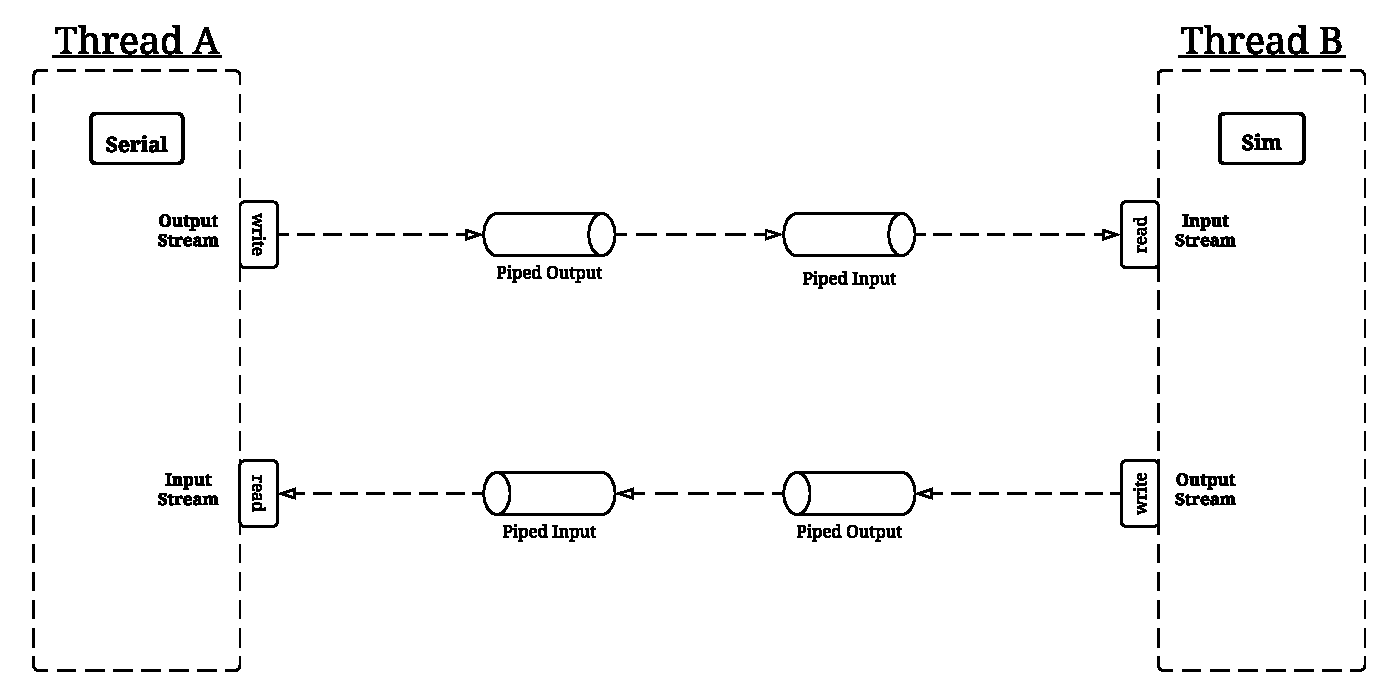
\includegraphics[width=1\textwidth]{fig/ainf/Pipe.pdf}
\caption{Kommunikation Producer-Consumer}
\label{ProducerConsumer}
\end{figure}
Hierbei ist zu bemerken, dass sich die Klasse, welche Daten an den Simulator überträgt,\\\lstinline[style=java]{SimInputStreamBuffer} benennt.
Das Gegenstück dazu ist die Klasse \lstinline[style=java]{SimOutpuStreamBuffer}.
In diesen beiden Klassen werden die jeweiligen \lstinline[style=java]{PipedInputStreams} und \lstinline[style=java]{PipedOutputStreams} gesetzt.
So ist nun die Verbindung zwischen beiden Threads hergestellt.
\subsection{Logging}
\subsubsection{Konzept}\label{sssec:logOverview}
Logging ist nach dem Debugging selbst, ein weiteres wichtiges Mittel um einzelne Programmbausteine oder das gesamte Programm auf Fehler zu untersuchen.
Mithilfe einer Log-Datei können z.B aktuelle Wertebelegungen im Detail dargestellt werden.
Natürlich kann dies auch mithilfe einer Konsolenausgabe über \lstinline[style=java]{System.out.println()} realisiert werden, jedoch ist eine Verwendung von Logging-Frameworks aufgrund der Flexibilität im Einsatz immer sinnvoller.

\textbf{Gründe für die Verwendung von Logging-Frameworks}\\
Als Beispiel kann mithilfe einer Log-Datei auch ein Benutzer, welcher nicht über die Möglichkeit verfügt, den Quellcode einzusehen, einzelne Fehler erkennen (vorausgesetzt diese Möglichkeit ist durch das Programm geschaffen).
Außerdem ist nun die Persistenz der Logging-Einträge gegeben.
Dies bedeutet, es kann nun sichergestellt werden, dass diese Einträge auf dem System gespeichert werden und nach einem Neustart verfügbar sind.
Nutzt man diese Art von Protokollierung, kann man außerdem die Genauigkeit der Erfassung genau parametrisieren.\\
Zusammengefasst bringt das Erstellen einer Log-Datei mithilfe eines Logging-Frameworks ein großes Feld an Möglichkeiten mit sich.\\\\
\subsubsection{Integration in das Programm}
\footfullcite[Vgl.][]{Steiner2020}Aufgrund der gegebenen Klassen, welche das Logging implementieren, ist die Integration in das Programm einfach umzusetzen.
Es ist lediglich notwendig, diese genannten Klassen in ein Package des Programms einzufügen.
Dazu soll in der \autoref{PackagestrukturLogging} die Struktur des Logging-Packages illustriert werden.
\begin{figure}[H]
\begin{center}
\begin{forest}
for tree={
font=\ttfamily,
grow'=0,
child anchor=west,
parent anchor=south,
anchor=west,
calign=first,
edge path={
\noexpand\path [draw, \forestoption{edge}]
(!u.south west) +(7.5pt,0) |- node[fill,inner sep=1.25pt] {} (.child anchor)\forestoption{edge label};
},
before typesetting nodes={
if n=1
{insert before={[,phantom]}}
{}
},
fit=band,
before computing xy={l=15pt},
}
[logging
[ExtendedLogRecord]
[LogBackgroundHandler]
[LogOutputStreamHandler]
[LogRecordData]
[LogRecordDataFormattedText]
[LogRecordDataHexDump]
[LogRecordDataString]
[Logger]
]
\end{forest}
\end{center}
\caption{Packagestruktur-Logging}
\label{PackagestrukturLogging}
\end{figure}
Um nun die Implementierung zu vervollständigen, muss nun in der Main-Methode, welche im Package \lstinline[style=java]{main} zu finden ist, der Logger parametrisiert werden.

Im Gegensatz zu Javas Standard-Logger-Objekt sind alle Logger-Objekte automatisch an einen einzigen "übergeordneten" Logger gebunden.
Nun ist es zuallererst nötig, das Binding eines Handlers an das "übergeordnete" Logger-Objekt durchzuführen.
Dies erfolgt mithilfe der Zeile \lstinline[style=java]{private static final Logger LOGP = Logger.getParentLogger()}.\\
Der genannte Logger soll nun dessen Protokollierung auf zwei verschiedenen Ausgaben schreiben.
\begin{enumerate}
\item Konsolenausgabe
\item Log-Datei
\end{enumerate}
Um diese Anforderung zu erfüllen, ist es notwendig den Logger mithilfe der folgenden Zeilen im \autoref{loggerOutput} zu konfigurieren.
% @formatter:off
\begin{lstlisting}[style=java,caption=Logger Implementierung,label=loggerOutput]
LOGP.addHandler(new LogBackgroundHandler(
    new LogOutputStreamHandler(System.out)));
try {
    LOGP.addHandler(new LogBackgroundHandler(
        new LogOutputStreamHandler(new FileOutputStream(logPath))));
}
catch (FileNotFoundException ex) {
    System.out.println("Should not see me :)");
}
\end{lstlisting}
% @formatter:on
Nun kann der Logger global im Programm angewendet werden.
Es ist nur mehr nötig, dieses Logger-Objekt in die jeweilige Klasse zu bringen.
Dies erfolgt über die Zeile \lstinline[style=java]{private static final Logger LOG = Logger.getLogger(Example.class.getName())}.
In diesem Beispiel wird das Logger-Objekt der Klasse \lstinline[style=java]{Example} zugewiesen.\\\\
Wie schon im \autoref{sssec:logOverview} beschrieben, ist durch einen Logger die Möglichkeit gegeben, eine verschieden genaue Darstellung von Einträgen zu implementieren.\\
Folgend soll tabellarisch gezeigt werden, welche Möglichkeiten dieser Logger bietet.
\begin{table}[H]
\centering
\begin{tabular}{|l|l|l|}
\hline
\rowcolor[HTML]{FFFFFF}
\textbf{Methodenname} & \textbf{Schlüsselwort} & \textbf{Beschreibung}                                                                                                \\ \hline
\rowcolor[HTML]{FFFFFF}
DEBUG                 & debug                  & Verwendete Darstellung während Development                                                                          \\ \hline
SEVERE                & severe                 & \begin{tabular}[c]{@{}l@{}}Verwendung bei gravierenden Fehler \\ mit großer Auswirkung auf das Programm\end{tabular} \\ \hline
WARNING               & warning                & \begin{tabular}[c]{@{}l@{}}Verwendung bei kleinen Fehlern welche\\ keine große Auswirkung haben\end{tabular}         \\ \hline
INFO                  & info                   & Verwendung bei normalen Ausgaben                                                                                     \\ \hline
CONFIG                & config                 & Verwendung bei Konfigurationen                                                                                                                       \\ \hline
FINE                  & fine                   & Genaue Darstellung von Nachrichten                                                                                   \\ \hline
FINER                 & finer                  & Genauere Darstellung von Nachrichten                                                                                 \\ \hline
FINEST                & finest                 & Genaueste Darstellung von Nachrichten                                                                                \\ \hline
ALL                   & all                    & Darstellung von allen Nachrichten                                                                                    \\ \hline
\end{tabular}
\caption{Logger-Funktionen}
\end{table}
\subsection{Konfigurationsdatei}\label{subsec:konfiguration}
\subsubsection{Konzept}
Sollten, wie in unserem Fall, Daten über einen längeren Zeitpunkt gespeichert werden und diese auch nach einem Systemneustart noch verfügbar sein, kann eine Datei implementiert werden, welche diese Daten speichert.
In unserem Fall beziehen sich diese Daten auf Konfigurationseinträge der Maschine.
Einige Anforderungen an diese Konfigurationsdatei sind:
\begin{enumerate}
\item Textuell
\item Einfache Erweiterbarkeit
\item Übersichtliche Darstellung
\end{enumerate}
Aufgrund dieser Darstellung soll eine Lösung mithilfe des Datenformats JSON geschaffen werden.
Nun ergibt sich jedoch das Problem, dass eine enorm große Datenmenge in dieses Objekt verpackt werden muss.
Eine Lösung bietet, wie im \autoref{sssec:json} erwähnt, die Bibliothek Gson.
Diese vereinfacht die Erstellung einer Json-Datei.
Somit kann in wenigen Schritten dieses Ziel umgesetzt werden.
\subsubsection{Umsetzung}
Die Realisierung dieser Config-Datei erfolgt voll und ganz in der Klasse \lstinline[style=java]{Config} welche als Singelton implementiert wird.
Diese genannte Klasse stellt lediglich Setter-Methoden zum Setzten der Einträge sowie die Methode \lstinline[style=java]{save()} zur Verfügung.
Nach einem Aufruf der genannten Methode \lstinline[style=java]{save()} wird die aktuelle Instanz der Config-Datei auf dem System an einem gewissen Pfad gespeichert.
Dieser Pfad wird automatisch bei jedem Startvorgang des Programms, anhand von Untersuchungen verschiedener Plätzen im Dateisystem, festgelegt.
Diese typischen Plätze sollten vom Programm vorgegeben sein.
Falls nirgends die Möglichkeit besteht, diese Datei zu schreiben, wird im Projektverzeichnis automatisch eine Datei angelegt und daraufhin das Programm gestoppt, um diese nach dem auf GitHub verfügbaren Pattern abzuändern.
Dieses Pattern soll kurz in der \autoref{sampleConfig} gezeigt werden.
\begin{lstlisting}[style=json, caption=JSON-Codebeispiel,label=sampleConfig]
{
    "logPath": "",
    "statisticsPath": "",
    "guiHeight": 600,
    "guiWidth": 1024,
    "gamemodes": [
    ],
    "serial": {
        "disabled": false,
        "device": "sim",
        "baudrate": 57600,
        "timeoutMillis": 1000,
        "secondTryAllowed": false,
        "responseByteLength": 32
    },
    "internationalization": {
        "language": "en",
        "country": "US",
        "bundlePath": "",
        "bundlePrefix": "bundle"
    }
}
\end{lstlisting}
Des Weiteren sollte das Einlesen dieser Konfigurationsdatei im privaten Konstruktor nicht unerwähnt bleiben.
Dies bedeutet, dass sobald die Methode \lstinline[style=java]{createInstance()} aufgerufen wird, ein vollwertiges Objekt der Konfigurationsdatei zur Verfügung steht.
Dieses genannte Objekt ist eine Instanz der Datenerhaltungsklasse \lstinline[style=java]{ConfigModel}.\\\\
Implementiert wird das Einlesen durch die Methode \lstinline[style=java]{read()}, welche über einen \lstinline[style=java]{BufferedReader} den JSON-String einliest.
Dieser String wird anschließend, wie im Kapitel \nameref{sssec:json} schon geklärt, in dieses genannte Objekt umgewandelt.\\
So verfügt das Programm nun die Möglichkeit, wichtige Daten zu speichern und diese global innerhalb der Programms abzurufen.
\subsection{Statistiken}
\subsubsection{Konzept}
Sobald die Implementierung der Konfigurationsdatei abgeschlossen ist, kann nun nach dem gleichen Schema auch die Statistik-Datei erstellt werden.\\\\
Diese genannte Datei soll nach jedem Beenden des aktuellen Spiels, was mithilfe eines Buttons am Interface realisiert wird, neu geschrieben werden.
Die Bestandteile dieser Datei sollten vor der Umsetzung klar definiert sein.
\begin{enumerate}
\item Gesamtanzahl aller Spiele
\item Jedes einzelne Spiel
\begin{enumerate}
\item Alle Spielernamen und deren Punktestand
\item Den gespielten Spielmodus mit dessen Hintergrundinformationen
\end{enumerate}
\end{enumerate}
\newpage
\subsubsection{Umsetzung}
Wie schon genannt, erfolgt die Umsetzung genau nach dem gleichen Schema wie das der Konfigurationsdatei aus dem \autoref{subsec:konfiguration}.
Dies bedeutet, dass hier anstatt des \lstinline[style=java]{ConfigModel}, das \lstinline[style=java]{StatisticModel} die Basis der Datei darstellt.
Dieses Model verfügt eine Liste von Objekten des Typs \lstinline[style=java]{GameModel}, welches den Kopf eines jeden Spiels visualisiert.
Außerdem beinhaltet es einen Zahlenwert zur Zählung der gespielten Spiele.\\\\
Ab diesem Zeitpunkt ist es nun möglich, Statistiken des gesamten Lebenszykluses der Maschine, in einer Datei darzustellen.
Dies soll im \nameref{sssec:statsController} an Bedeutung und Relevanz gewinnen.
\newpage
\section{Frontend-Programmierung}
In dem folgenden Kapitel wird näher über das sogenannte "Frontend" gesprochen.
Die Definition des Frontends bezieht sich in dieser Arbeit auf alle notwendigen Programmbausteine, welche zur Darstellung der grafischen Benutzeroberfläche notwendig sind.\\\\
So wird gezeigt, wie die grafische Oberfläche organisiert ist und wie diese mit den jeweiligen Controllern zusammenarbeitet.
Beschrieben werden jedoch nur wichtige Programmelemente und keine Grundlagen von JavaFX, da dies ansonsten den Rahmen sprengen würde.\\
Realisiert wurde die Oberfläche mithilfe von zwei verschiedenen Fenstern, auf welche anschließend in \autoref{subsec:startupController} und \autoref{subsec:mainController} eingegangen wird.
\subsection{Designkonzept}
Aufgrund des großen Spektrums an gebotenen Möglichkeiten, soll eine grafische Oberfläche gebaut werden, welche alle Anforderungen aus dem \autoref{subsec:fronted-programmierung} erfüllt.
Sobald es aber jetzt, wie in den Anforderungen, um den Bereich der User-Experience geht, kommt man an der von Google entwickelten Designsprache namens Material-Design nicht vorbei.
Folgend soll der Vergleich von Material-Design und Flat-Design gezeigt werden.\\\\
\footfullcite[Vgl.][]{kulturbanause2016}
Grundlegend besteht der Look von Material Design aus farbigen Flächen, einfachen Icons und großen Bildern, welche auf einer aufgeräumten Interaktionsoberfläche angezeigt werden.
So wird dieses Design jedoch oft mit dem Flat-Design verwechselt aber
es bestehen wesentliche Unterschiede.
Im Gegensatz zum Flat Design, wo es hauptsächlich um die Ästhetik und Reduzierung der Oberfläche geht, spielt beim Material Design die Optimierung der Benutzerfreundlichkeit sowie die Implementierung von physikalischen Gesetzen eine wichtige Rolle.
Jedoch ist auch zu beachten, dass beim Material Design eine virtuelle Z-Achse geschaffen wird um Dreidimensionalität zu kreieren.
Auch besteht ein weiteres Ziel darin, viel mit Animationen, animierten Übergängen, sowie Licht und Schatten zu arbeiten.
So sollte sich bei der Erstellung an folgender Grafik gehalten werden.
\begin{figure}[H]
\centering
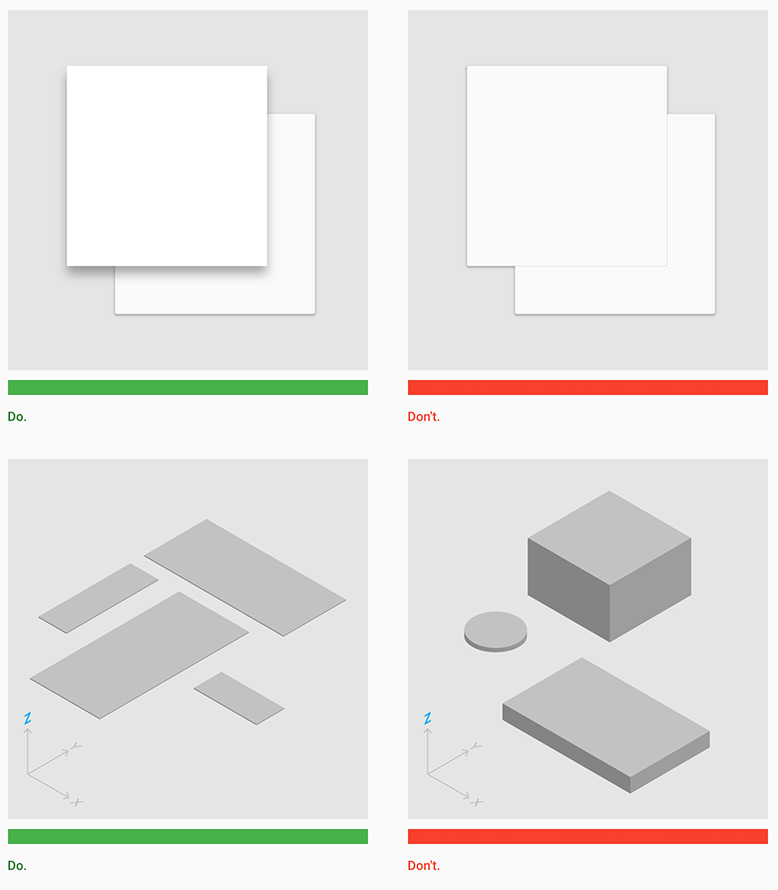
\includegraphics[width=0.5\textwidth]{fig/ainf/material-design-rules.png}
\caption{Material-Design Vorgaben}
\label{rpiAndDisplay}
\end{figure}
Mithilfe dieser Hintergrundinformation steht jetzt der Erstellung der grafischen Oberfläche nichts mehr im Wege.
\subsection{MVC-Implementierung}\label{subsec:mvc}
Wie schon in der Beschreibung von JavaFX erwähnt, kann die grafische Oberfläche nach dem MVC-Pattern organisiert werden.
So ist es nun nötig, Design und Funktionalität voneinander zu trennen, und dessen Verknüpfung auch erst nachträglich im Programmcode zu vollziehen.
Würde man es genau nehmen, dürften noch nicht einmal Controller-Klassen in diesen FXML-Dateien genannt werden.\\\\
Wichtig ist jetzt auch, das sogenannte Event-Handling sowie die Verknüpfung wischen FXML und Controller-Klassen programmatisch vorzunehmen.\\\\
\textbf{Anpassungen innerhalb des Controllers}\\
Mithilfe der Implementierung des Interface \lstinline[style=java]{Initializable} ist es möglich die Methode \lstinline[style=java]{initialize()} zu erzeugen.
Diese wird nach jedem Start des Programms automatisch aufgerufen.
In dieser können nun etwaige Events definiert werden.
% @formatter:off
\begin{lstlisting}[style=java,caption=Methode initialize(),label=loggerOutput]
@Override
public void initialize(URL arg0, ResourceBundle arg1) {
    btDelete.setOnAction(this::handleDelete);
}
\end{lstlisting}
% @formatter:on
\textbf{Anpassungen beim Startvorgang}\\
Nun muss nur noch der explizite Controller beim Starten definiert werden.
% @formatter:off
\begin{lstlisting}[style=java,caption=Methode start(),label=loggerOutput]
@Override
public void start(Stage stage) {
try {
    final FXMLLoader fxmlLoader = new FXMLLoader(fxmlUrl,
        ResourceManager.getInstance().getCurrentRecourceBundle());
    fxmlLoader.setController(new StartupController());
    final Parent root = fxmlLoader.load();
    stage.setScene(new Scene(root, Config.getInstance().getGuiWidth(),
        Config.getInstance().getGuiHeight()));
    stage.initStyle(StageStyle.UNDECORATED);
    stage.setTitle("Startup GUI");
    stage.show();

    LOG.info(stage.getTitle() + " started successfully");
} catch (IOException ex) {
    LOG.severe("Exception while running GUI" + ex);
}
\end{lstlisting}
% @formatter:on
\textbf{Fazit}\\
So ist es nun möglich, mit wenigen Schritten diese genannte Trennung sauber durchzuführen.
Diese soll in allen weiteren Programmabschnitten vollzogen werden.
\subsection{Startup-Window und Controller}\label{subsec:startupController}
Aufgabe des Startup-Windows ist es, den Benutzer das Spiel, welches er spielen möchte, parametrisieren zu lassen.
Diese Parametrisierung beinhaltet das Auswählen eines Spielmodus sowie die Konfiguration der Spielernamen.\\\\
Die Auswahl eines Spielmodis erfolgt über eine eigens dafür bereitgestellte ComboBox.
In dieser ComboBox befinden sich Objekte vom Typ \lstinline[style=java]{GamemodeModel}, gezeigt im \autoref{gamemodeModel}.
Hierbei wurde von der Annotation \lstinline[style=java]{@SerializedName} gebrauch gemacht, welche das Datenelement mit einem bestimmten Namen in die JSON-Datei schreibt.
So ist das Annotation Attribut genau der Name des Elements in der Datei.
\lstinputlisting[firstline=7, lastline=16, style=java,caption=Klasse GamemodeModel(),label=gamemodeModel]{src/data/model/GamemodeModel.java}
Sollte nun der Spieler nicht zufrieden mit gegebenen Spielmodis aus der ComboBox sein, kann er diese selbst auf ihn abstimmen und konfigurieren.
Es kann hier über das Interaktionsmenü die Karten-, Spieler-, und Automatic-Deal-Anzahl (AutoDeal) eingestellt werden.
Außerdem kann der Name des Spielmodis verändert werden.
Ist dies der Fall, führt das zu einer Ergänzung eines neuen Spielmodis mit den eingestellten Parametern in der eigens dafür vorgesehenen Konfigurationsdatei.\\\\
So ist, wie oben schon erwähnt, die Möglichkeit gegeben, Spielernamen zu bearbeiten.
Dies wird durch die Liste in \autoref{startupWindow} ersichtlich.
Wird in dieser Liste ein Spielername selektiert, übernimmt das Programm diesen direkt in das darüber befindliche Textfeld.
Von dort aus kann der Name bearbeitet werden.\\
Umgesetzt wird dies mithilfe von zwei sogenannte \lstinline[style=java]{ChangeListeners}, welche dauerhaft auf eine Veränderung, also einen "Change" warten, um dann eine Methode auszuführen.
Neben Listener wären auch Properties und Bindings für diese Anwendung möglich.
Besser sind jedoch Listener.
%\lstinputlisting[firstline=54, lastline=59, style=java,caption=Deklaration ChangeListener,label=changelistener]{src/gui/controller/StartupController.java}
% @formatter:off
\begin{lstlisting}[style=java,caption=Deklaration ChangeListener,label=changelistener]
private final ChangeListener<String> nameChangeListener
    = (observableValue, oldValue, newValue) -> {
    notifyList(newValue);
};
private final ChangeListener<PlayerModel> playerListener
    = (observableValue, oldValue, newValue) -> {
    tfPlayerName.setText(newValue.getName());
};
\end{lstlisting}
% @formatter:on
\footfullcite[Vgl.][]{Oracle2015}Folgend wird auf eine Besonderheit bei der Füllung der ComboBox und der Liste eingegangen.
Wie schon in Java-Swing, kann auch in JavaFX die Darstellung der Daten einer Tabelle oder einer Liste flexibel angepasst werden.
Grund für die Verwendung solcher Mechanismen ist das Problem der erheblichen Speicherverschwendung bei der Anzeige.
So werden nicht alle Daten direkt verarbeitet, sondern nur Daten, welche wirklich auf dem Bildschirm dargestellt werden.
Außerdem hat solch ein Verfahren den Vorteil, dass nun die Darstellung von Datenelementen eines Objekts spezifischer abgestimmt werden kann.
Zu sehen ist dies in der \autoref{CellRendering}.
\begin{figure}[H]
\centering
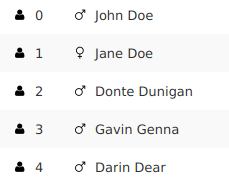
\includegraphics[width=0.3\textwidth]{fig/ainf/CellRendering}
\caption{Cell-Rendering Beispiel}
\label{CellRendering}
\end{figure}
Umgesetzt wird dies mithilfe der Basisklasse \lstinline[style=java]{javafx.scene.control.Cell}.
Im \autoref{CellFactory} wird im ersten Schritt die Darstellung einer einzelnen Zelle definiert.
\lstinputlisting[firstline=302, lastline=313, style=java,caption=Klasse PlayerCell(),label=CellFactory]{src/gui/controller/StartupController.java}
Jetzt muss lediglich die CellFactory mithilfe des Methodenaufrufs \lstinline[style=java]{playerNameList.setCellFactory(list -> new PlayerCell())} gesetzt werden und die Liste baut sich nach dem Import der Daten zusammen.
Genau das gleiche Verfahren kann auch bei der ComboBox angewendet werden.\\\\
\begin{figure}[H]
\centering
\vspace{-10mm}
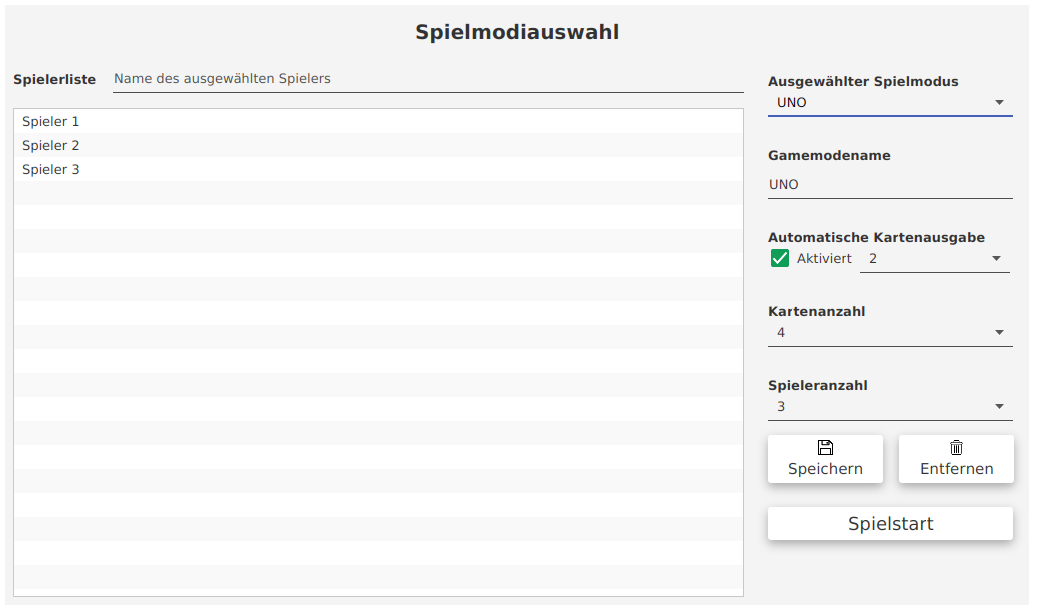
\includegraphics[width=0.8\textwidth]{fig/ainf/Startup_German.png}
\caption{Startup-Window}
\label{startupWindow}
\end{figure}
\subsection{Main-Window und Controller}\label{subsec:mainController}
Das Main-Window stellt im engsten Sinne das Interaktionsfenster des Benutzers während des Spiels dar.
Dieses wird mithilfe von Tabs realisiert.
Jeder einzelne Tab besitzt einen eigenen Controller.
Aufgrund dieser Strukturierung ist der Code viel durchschaubarer und strukturierter.
Die Verlinkung kann ganz einfach innerhalb der FXML-Dokumente geschehen.
\begin{figure}[H]
\centering
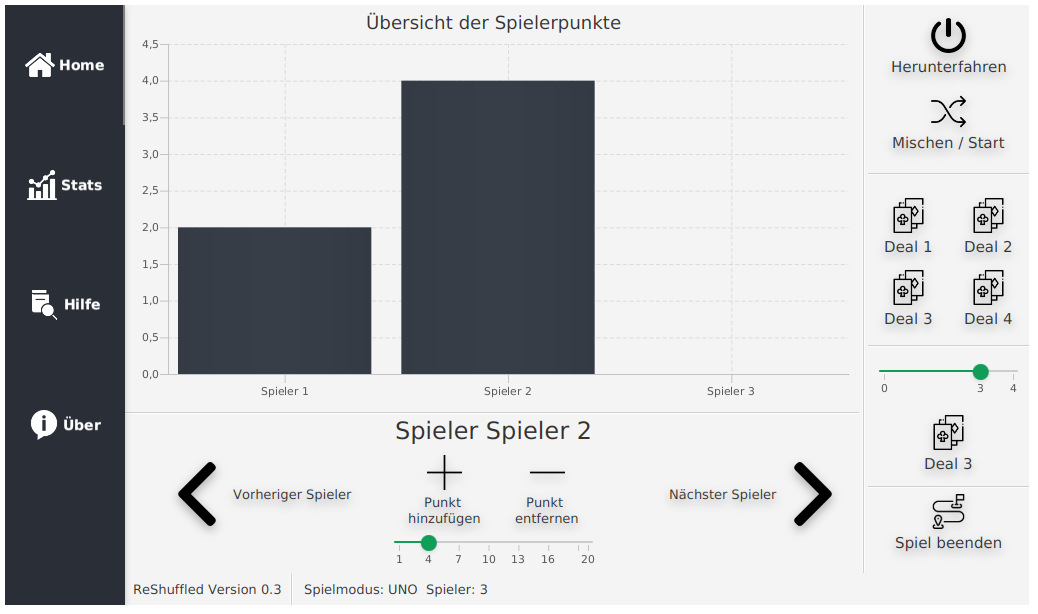
\includegraphics[width=0.8\textwidth]{fig/ainf/Main_Home_German.png}
\caption{Main-Window}
\label{mainWindows}
\end{figure}
In den folgenden Kapiteln wird nun jeder einzelne Tab beschrieben und gezeigt, welche Besonderheiten er an Code mit sich bringt.
\subsection{Home-Tab und Controller}
Zuerst springt einen sofort der Home-Tab ins Auge.
Dieser fällt sofort mit der mittig platzierten Punkteanzeige auf.
Mithilfe der zwei Buttons, nämlich \textit{Vorheriger Spieler} und \textit{Nächster Spieler}, kann zwischen den Spielern gewechselt werden.
Adaptiv kann jedem Spieler jetzt ein Punkt hinzu oder abgezogen werden.
Sollte je ein Punkt nicht ausreichen, kann mithilfe eines implementierten Sliders eine größere Anzahl an Punkten zugewiesen werden.\
Wird ein Punkt hinzugefügt, aktualisiert dies automatisch die Punkteanzeige.\\\\
Umgesetzt wurde diese genannte Anzeige als \lstinline[style=java]{XYChart}, welcher mithilfe der folgenden Zeilen deklariert wurde.
\lstinputlisting[firstline=42, lastline=45, style=java,caption=Initialisierung der Diagrammachsen,label=XYChart]{src/gui/controller/HomeController.java}
Nachdem diese Deklarierung erfolgt ist, kann mit der Methode \lstinline[style=java]{updateBarChart()} die Grafik aktualisiert werden.
Diese Methode iteriert durch alle Spieler des Game-Objekts, holt die Namen sowie Punkteanzahl der Spieler heraus und schreibt sie in den \lstinline[style=java]{XYChart}.\\
Neben dieser Funktion stellt das Dashboard auf der linken Seite ein Kontrollmenü zum Steuern der Maschine bereit.
In diesem Menü kann mit einem Drücken auf den Button \textit{Herunterfahren} und dem anschließenden Bestätigen der Abfrage(\autoref{sssec:alert}), die Maschine heruntergefahren werden.
Im Hintergrund werden hier vom Backend, Daten über die serielle Schnittstelle gesendet.\\
Auf dem gleichen Prinzip basiert auch der Button \textit{Mischen}, nur dass dieser Karten mischen lässt und anschließend mithilfe der AutoDeal-Funktion, automatisch Karten ausgibt.\\
Sollen während des Spiels nur einzelne Karten benötigt werden, können mithilfe der Button-Group \textit{Deal} Karten ausgeteilt werden.
Diese können, wie auch bei der Punkteanzahl, mithilfe eines Sliders ausgewählt werden.
Das Programm deaktiviert nach dem Fehlen von vorhandenen Karten die Buttons und es ist erst nach einem weiteren Mischvorgang möglich, weiter auszuteilen.\\
\begin{figure}[H]
\centering
\vspace{-5mm}
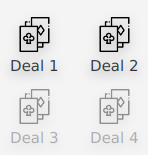
\includegraphics[width=0.2\textwidth]{fig/ainf/Interface.png}
\caption{Interaktionsmenü-Kartenausgabe}
\label{interface}
\end{figure}
Wird mit dem Button \textit{Spiel beenden} nun das Spiel beendet, wird vollautomatisch das Game-Objekt in die Statistik-Datei geschrieben.
Infolgedessen gelangt der Spieler wieder in das Startup-Window zurück.
So schließt sich der Zyklus eines Spieles wieder und es kann ein neues gestartet werden.
\subsection{\acs{Stats}-Tab und Controller}\label{sssec:statsController}
Der Stats-Tab bietet die Möglichkeit , Statistiken aus der Statistik-Datei abzurufen.
Diese genannten Daten werden innerhalb einer \lstinline[style=java]{TreeTableView<S,T>} angezeigt.
Aufgrund der Tatsache, dass eine \lstinline[style=java]{TreeTableView<S,T>} eines der komplexesten Bedienelemente in JavaFX ist, soll nun darauf eingegangen werden.\\\\
Eine \lstinline[style=java]{TreeTableView<S,T>} ist hierarchisch organisiert.
Das beutetet, dass das Datenmodell aus verschiedenen Instanzen, in unserem Fall Instanzen vom Typ \lstinline[style=java]{Game} besteht.
Diese werden in einer Gruppe zusammengefasst, welche wiederum in einer Hauptgruppe namens \lstinline[style=java]{root} zusammengefasst werden.
So besteht eine Baumstruktur.
Dargestellt werden die Daten über Instanzen vom Typ \lstinline[style=java]{TreeItem<T>}.
Erstellt werden diese TreeItems mithilfe der Methode \lstinline[style=java]{createTreeData())}.
\newpage
\lstinputlisting[firstline=43, lastline=56, style=java,caption=Methode createTreeData(),label=createTreeData]{src/gui/controller/StatsController.java}
In dieser Methode wird zuerst die Hauptgruppe namens \lstinline[style=java]{root} erstellt.
Im nächsten Schritt werden alle Game-Instanzen geholt und mithilfe der Methode \lstinline[style=java]{createGroupTreeItem()} in Gruppenelemente umgewandelt.
\lstinputlisting[firstline=59, lastline=61, style=java,caption=Methode createGroupTreeItem(),label=createGroupTreeItem]{src/gui/controller/StatsController.java}
Innerhalb dieser Schleife, welche diese genannten Gruppen erstellt, befindet sich eine weitere Schleife, welche zu den jeweiligen Gruppen die einzelnen Spieler in Form von Instanzen vom Typ \lstinline[style=java]{TreeItem<PlayerModel>} hinzufügt werden.
Diese werden als sogenannte \lstinline[style=java]{children} betitelt.
Im letzten Schritt muss nun nur mehr das Data Binding umgesetzt werden.
Dies erfolgt mithilfe des folgenden Listing.
\lstinputlisting[firstline=63, lastline=74, style=java,caption=Methode createColumn(),label=dataBindinh]{src/gui/controller/StatsController.java}
Hier wird mithilfe von Instanzen des Typs \lstinline[style=java]{TreeTableColumn<S,T>} die Verbindung zu den Spalten hergestellt.
Dabei ist \lstinline[style=java]{S} der Typ der Elemente von {TreeItem<S>}.
Zum Auslesen der Werte nutzt man Objekte vom Typ \lstinline[style=java]{TreeItemPropertyValueFactory}, welche man bei der Erstellung, den Namen des gewünschten Attributs übergibt.\\
Mithilfe dieses Codes ist es nun möglich, eine ansprechende TreeTableView zu bauen.
\subsection{About- und Help-Tab und Controllers}
Die nebensächlichen Tabs namens \textit{About} und \textit{Help} stellen lediglich einige Informationen für den Benutzer der Maschine bereit.
Diese wird in Form von Pfeilen und Texten beschriebenen Bildern dargestellt.
Im \textit{About-Tab} findet sich jedoch ein kleines Feature.
Mithilfe einer ComBox kann hier die gewünschte Systemsprache gewählt werden.
Die  wird im \autoref{sssec:internationalization} näher beschrieben.
So bieten diese beiden Tabs im Großen und Ganzen eine Schnittstelle zur Informationsbeschaffung für den Benutzer an.
\subsection{Alerts}\label{sssec:alert}
Um wie in JavaFX die Möglichkeit zu haben, Abfragen vorzunehmen, wurden in diesem Projekt sogenannte Dialoge implementiert.
Diese werden durch die Utility-Klasse \lstinline[style=java]{AlertUtil} bereitgestellt.
Mithilfe der implementierten Methode \lstinline[style=java]{showContentDialog()} kann ein Dialog erstellt werden.
Dieser erstellte Dialog wird mithilfe einer \lstinline[style=java]{StackPane} über das aktuelle Layout gelegt.
In der Parameterliste befindet sich also diese \lstinline[style=java]{StackPane} und wird innerhalb der Methode als \lstinline[style=java]{root} betitelt.
Aufgrund des zusätzlichen Features der Weichzeichnung des Hintergrunds,muss hier eine \lstinline[style=java]{Node} übergeben werden, auf welcher der Effekt angewendet werden soll.
Außerdem ist es nötig eine Liste von \lstinline[style=java]{JFXButton}, also den verwendeten Buttons, zu übergeben.
Zusätzlich muss ein Titel und ein Text angegeben werden.
\lstinputlisting[firstline=24, lastline=41, style=java,caption=Methode showContentDialog(),label=showContentDialog]{src/util/AlertUtil.java}
So führt der Aufruf der Methode zu einem Erstellen eines Dialogs.\\
Wird nun auf einen Button der übergebenen Liste ein EventHandler mithilfe der Methode \lstinline[style=java]{addEventHandler()} gesetzt,
kann auf das Schließen oder Bestätigen des Dialogs gewartet werden und danach eine spezifische Aktion erfolgen.
\begin{figure}[H]
\centering
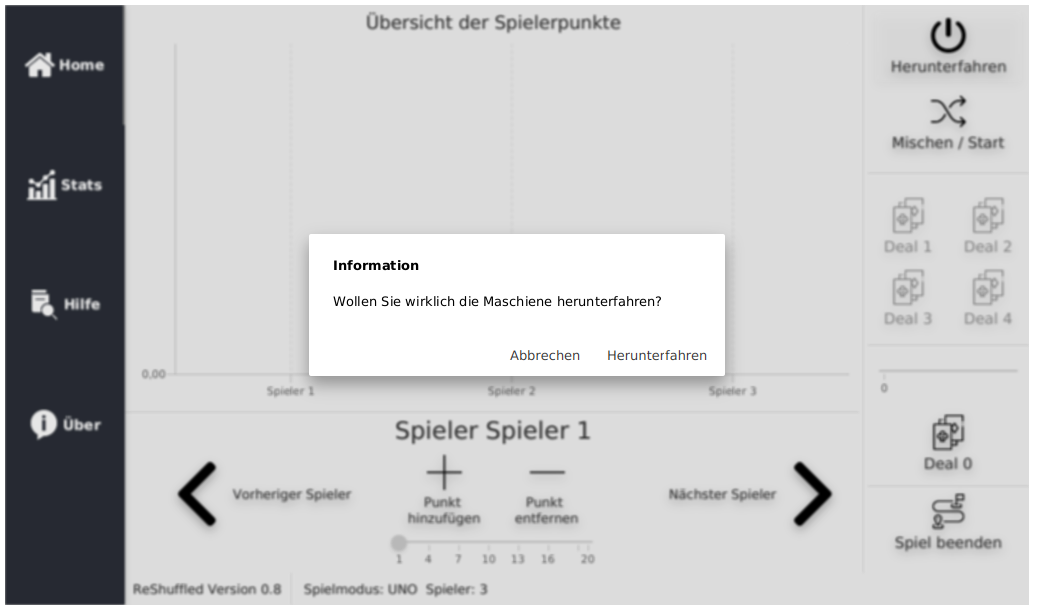
\includegraphics[width=0.8\textwidth]{fig/ainf/Shutdown-Dialog.png}
\caption{Dialog}
\label{shutdown}
\end{figure}
\subsection{Internationalisierung}\label{sssec:internationalization}
Um das Produkt in verschiedenen Ländern einsatzfähig machen zu können und den Benutzer das beste Erlebnis zu bieten, ist es notwendig, etwaige Texte, Uhrzeiten usw. der grafischen Oberfläche in das Format des spezifischen Landes zu konvertieren.
In JavaFX ist dies recht einfach umgesetzt.
Hier hilf die Klasse \lstinline[style=java]{Locale} bei der Beschreibung von etwaigen Sprachbesonderheiten.
Eine Instanz vom Typ \lstinline[style=java]{Locale} beinhaltet eine bestimmte geografische Region, sowie die in diesem Land gesprochene Sprache.
Die Darstellung innerhalb des Objektes ist von der ISO 639 und der ISO 3166 abgeleitet, welche eine einheitliche Kodierung von Länder-und Sprachcodes vorraussetzen.
Beim Erstellprozess einer Oberfläche kann nun dieses Local-Objekt als Parameter an den \lstinline[style=java]{FXMLLoader} übergeben werden.\\\\
Nun gibt es die Möglichkeit, Sprachdateien zu implementieren, welche alle übersetzten Texte beinhalten.
Diese Dateien sollte nach folgendem Pattern benannt werden: \lstinline[style=java]{prefix_<sprachkürzel>_<länderkürzel>.properties}\\
Innerhalb dieser Sprachdatei sind übersetzte Texte immer mit Konstanten verknüpft.
Gezeigt wird dies in folgenden Beispiel.
% @formatter:off
\begin{lstlisting}[style=java,caption=Beispielbundle,label=resource]
txt_about_save=Speichern
txt_home_player=Spieler
txt_home_gamemode=Spielmodus
txt_msg_finishGame=Wollen Sie wirklich das Spiel beenden?
\end{lstlisting}
% @formatter:on
Die folgende Methode filtert nun genau nach dem oben genannte Pattern und es werden infolgedessen die Daten eingelesen.
\lstinputlisting[firstline=17, lastline=20, style=java,caption=Methode getMatchingFiles(),label=readBundle]{src/util/FileUtil.java}
Sobald diese nun standardmäßig eingelesen wurden, kann aus diesen Daten ein Local erstellt werden welches anschließend mit der Methode \lstinline[style=java]{Methode activateLocale()} aktiviert werden kann.
\lstinputlisting[firstline=90, lastline=101, style=java,caption=Methode activateLocale(),label=multiLang]{src/gui/multilanguage/ResourceManager.java}
Diese Methode prüft zuerst mit \lstinline[style=java]{supportsLocale()}, ob das gewünschte Objekt überhaupt im Speicher vorhanden ist.
Sollte dies der Fall sein wird das Attribut \lstinline[style=java]{currentResourceBundle}, welches das aktuelle Bundle darstellt, gesetzt.
Im letzten Schritt ist es noch notwendig, in die Konfigurationsdatei das aktuelle Locale zu schreiben, um dann beim nächsten Start dieses zu verwenden.
\newpage
\section{Hardwarenahe-Programmierung}
Um nun die gesendeten Daten über der seriellen Schnittstelle auf der Ansteuerplatine zu erhalten, ist es notwendig, diese genannte Platine einzurichten und zu programmieren.
Im folgenden Abschnitt wird nun dieser Prozess näher erklärt.
\subsection{Konfiguration des Mikrocontrollers}
\footfullcite[Vgl.][]{mikrocontroller.net2020}Nach der Bereitstellung der Platine beginnt der Prozess der Einrichtung des Mikrocontrollers.
Dieser erwähnte Mikrocontroller benennt sich ATmega324PA.
Bei einem neuen µC ist es grundsätzlich notwendig im Datenblatt genau dieses µCs den Auslieferungszustand der Fuses zu ermitteln.
So werden beispielsweise die ATmega Prozessoren mit aktiviertem internen Oszillator ausgeliefert und man darf sich nicht wunden, wieso des Mikrocontroller nicht funktioniert.
Aufgrund der Verfügbarkeit eines Programmiersteckers ist es nun einfach, diese Fuse-Bits, also die Bits, welche für die Konfiguration des Mikrocontrollers dienen zu setzten.
Verwendet wurde hierbei das Konsolenprogramm AVR-Dude und ein handelsübliches Programmiergerät.
\footfullcite[Vgl.][]{Haemmerling2020}Mithilfe eines Fuse-Calculators werden nun alle gewünschten Parameter, welche in der \autoref{fuses} verfügbar sind, angewählt und es wird eine Zeichenkette generiert.
\begin{figure}[H]
\centering
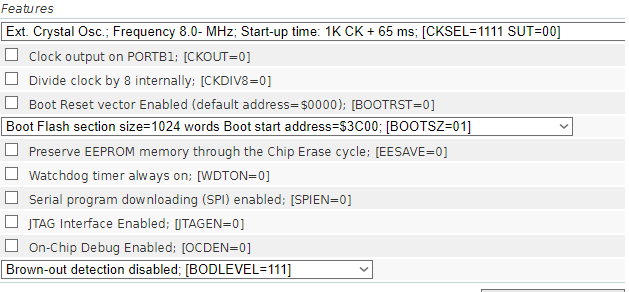
\includegraphics[width=0.8\textwidth]{fig/ainf/Features.PNG}
\caption{Fuse-Calculator}
\label{fuses}
\end{figure}
Diese Zeichenkette kann jetzt mithilfe von AVR-Dude verarbeitet werden.
% @formatter:off
\begin{lstlisting}[style=java,caption=Java-Codebeispiel,label=resource]
avrdude -c usbasp -P /dev/ttyUSB0 -p atmega324pa -e -U lfuse:w:0xfe:m
avrdude -c usbasp -P /dev/ttyUSB0 -p atmega324pa -e -U hfuse:w:0xd0:m
avrdude -c usbasp -P /dev/ttyUSB0 -p atmega324pa -e -U efuse:w:0xfe:m
\end{lstlisting}
% @formatter:on
Werden diese Fuse-Bits gesetzt, kann nun mithilfe von AVR-Dude ein Bootloader auf den Microcontroller gespielt werden.
So steht nun der volle Umfang des Mikrocontrollers zur Verfügung.
\subsection{Umsetzung Kommunikation} \label{ssec:konzeptCardDeal}
Sobald jetzt der Mikrocontroller programmierbar gemacht wurde, kann mit dem programmatischen Teil gestartet werden.
Ziel ist es, die serielle Kommunikation am Mikrocontroller zu realisieren.
Umgesetzt wurde dies mit verfügbaren Vorlagen, welche aus dem Unterricht bekannt waren.
In diesen Vorlagen sind etwaige Dinge, wie die Implementierung von Tasks oder UART schon vorkonfiguriert.
Dies erleichtert den Programmiervorgang enorm und führt zu einer schnelleren Umsetzung der Ziele.\\
Grundlegend muss jetzt die Verarbeitung der Daten und das Senden einer Antwort realisiert werden.
Das bedeutet, diese sollten in einem Buffer gespeichert und anschließend geprüft werden.
Wird ein Zeichen von der serielle Schnittstelle empfangen, wird die Funktion \lstinline[style=C]{app_handleUartByte()} aufgerufen.
\lstinputlisting[firstline=141, lastline=166, style=c,caption=Funktion apphandleUartByte(),label=multiLang]{src/app.c}
Zuerst wird geprüft, ob das erste ankommende Byte ein Startbyte also ein \lstinline[style=C]{:} ist.
Falls dies nicht der Fall, ist sollte der \lstinline[style=C]{ErrorCount} hochgezählt werden.
Wenn im Buffer bereits ein Startbyte : vorhanden ist, darf kein Zweites innerhalb der Request geschrieben werden, da dies sonst zu Fehlern führen könnte.
Falls ein solcher Fehler auftritt, sollte in einer Funktion ein weiteres mal der \lstinline[style=C]{ErrorCount} hochgezählt werden.
Werden danach mehr Zeichen in den Buffer geschrieben als Platz ist, wird ebenfalls der \lstinline[style=C]{ErrorCount} hochgezählt.\\
Ist nach dem Übertragen der \lstinline[style=C]{ErrorCount} größer als null, so soll die Anzahl der Fehler ausgegeben werden.
Verwendet wird hierbei eine LED auf dem Board.\\
Nachdem der Buffer gefüllt ist, wird die Funktion \lstinline[style=C]{app_handleModbusRequest()} aufgerufen die sich jetzt um diese Anfrage kümmert.
Die Aufgaben der Funktion sind folgende:
\begin{enumerate}
\item Prüfen auf validen Protokoll Request
\item Prüfen des CRC
\item Senden eines Response
\end{enumerate}
Mithilfe dieser beiden Funktionen ist es nun möglich, Requests zu Empfangen und eine Response zu schicken.
\newpage
\section{Teilaufbau}
Der letzte Schritt dieses Projekts ist es, einen Teil der Maschine aufzubauen.
Der Teilaufbau der Maschine gliedert sich in Display, Ansteuerplatine und Raspberry Pi.
Außerdem soll gezeigt werden, wie die Konfiguration des Display und das aufsetzten des Betriebssystems vonstatten ging.
\subsection{Konfiguration des Zielsystems}
\subsubsection{Betriebssystem}
Als Betriebssystem wurde Raspbian ausgewählt.
Das offizielle Betriebssystem für den Raspberry Pi basiert auf einem Debian-System mit Linux-Kernel.
Außerdem bringt es die aktuellste Unterstützung von Hardware mit und ist zudem noch außerordentlich schlank.
So wird auch der verwendete Display optimal Unterstützt.\\
Installiert werden kann Raspbian nach dem Download von der offiziellen Website.
Diese Installation startet mit dem erstellen einer Bootfähigen SD-Karte.
Ist nun die SD-Karte bootfähig, muss lediglich der Raspberry Pi gestartet werden.
Anschließend folgt eine Systemkonfiguration.
\subsubsection{Integration des Touchpanels}
Die Integration des Touchpanels ist spielt eine elementare Rolle bei der Inbetriebnahme der Maschine.
Ohne dieses Touchpanel kann nämlich kein Benutzer die Maschine bedienen.
Das ausgewählte Touchpanel besitzt folgende Eigenschaften:
\begin{enumerate}
\item  1024×600 Auflösung
\item Mit kapazitiven Touchcontrol
\item Einfache Konfiguration\\
Nach dem Anschließen muss nur mehr die \textit{config.txt}, welche sich im Root-Verzeichnis des Betriebssystems vom Raspberry Pi befindet, ergänzt werden.
Folgende Zeilen werden vorausgesetzt:
% @formatter:off
\begin{lstlisting}[style=java,caption=Display-Parameter,label=resource]
hdmi_force_hotplug=1
max_usb_current=1
hdmi_group=2
hdmi_mode=1
hdmi_mode=87
hdmi_cvt 1024 600 60 6 0 0 0
hdmi_drive=1
\end{lstlisting}
% @formatter:on
Ab diesem Zeitpunkt ist eine Verwendung des Displays möglich.
\subsubsection{Aufbau}
Das Ziel des letzten Schritts ist es, alle Komponenten miteinander zu verbinden.
Das bedeutet es muss noch die ausständige Verbindung der Ansteuerplatine und des Raspberry gemacht werden.
Diese wurde über einen 40 Pin Stecker realisiert, welcher alle Pins des Raspberry Pi auf die Ansteuerplatine führt.
So ist nun die serielle Verbindung sowie die Spannungsversorgung des Raspberry Pi sichergestellt.
\end{enumerate}
\begin{figure}[H]
\centering
\includegraphics[width=0.8\textwidth]{fig/ainf/IMG_3107.jpg}
\caption{Teilaufbau - Nicht bestromt}
\label{rpiAndDisplay}
\end{figure}
Um nun das gesamte System in Betrieb zu nehmen, ist es lediglich notwendig, eine Spannungsversorgung an die Ansteuerplatine anzuschließen.\\
Anhand dieses Stadiums können jetzt alle Komponenten in das Gehäuse eingebaut und verwendet werden.
\newpage
\section{Probleme - Verbesserungsmöglichkeiten - Zusammenfassung}
Im folgenden Abschnitt soll auf die entstandenen Probleme, welche während den Arbeiten aufgetreten sind, sowie den zukünftigen Verbesserungsmöglichkeiten eingegangen werden.
Schlussendlich soll eine kurze Zusammenfassung das Projekt abrunden.
\subsection{Probleme}
\subsubsection{Probleme bei der Implementierung von JavaFX}
Als erstes soll auf das Problem der Implementierung von JavaFX eingegangen  werden.
So ist es zu Beginn der Arbeiten nicht möglich gewesen, die Oberfläche der JavaFX-Applikation korrekt auf dem Interface, welches an den Raspberry Pi angeschlossen ist, anzeigen zu lassen.
Grund dafür ist die fehlende Unterstützung des JavaFX-Paketes innerhalb der offiziellen Java-Bibliothek.
Deswegen muss, laut der OpenJFX-Dokumentation (https://openjfx.io/openjfx-docs/), eine externe SDK für JavaFX heruntergeladen und als sogenanntes Module in die IDE implementiert werden.
Außerdem ist es nötig, diese SDK innerhalb der generierten \lstinline[style=C]{*.jar}-Datei zu implementieren.
Dies erfolgt in der Datei \lstinline[style=C]{build.xml} welche sich im root-Ordner befindet.
% @formatter:off
\begin{lstlisting}[style=xml,caption=Teilabschnitt build.xml,label=build]
<target name="-post-jar">
    <jar jarfile="dist/ReShuffled_PI-withLibs.jar">
        <zipfileset src="${dist.jar}" excludes="META-INF/*" />
        <zipfileset src="lib/jssc-2.8.0.jar" excludes="META-INF/*" />
        <zipfileset src="lib/gson-2.8.6.jar" excludes="META-INF/*" />
        <zipfileset src="lib/jfoenix-9.0.8.jar" excludes="META-INF/*" />
        <zipfileset src="lib/javafx.base.jar" excludes="META-INF/*" />
        <zipfileset src="lib/javafx.controls.jar" excludes="META-INF/*" />
        <zipfileset src="lib/javafx.fxml.jar" excludes="META-INF/*" />
        <manifest>
            <attribute name="Main-Class" value="main.Main"/>
        </manifest>
    </jar>
    <move file="dist/ReShuffled_PI-withLibs.jar" tofile="dist/ReShuffled_PI.jar" />
</target>
\end{lstlisting}
% @formatter:ongenannt
Nun ist es mithilfe dieser wenigen Zeilen möglich, alle Abhängigkeiten in diese jar-Datei zu implementieren und diese Datei am Raspberry Pi nach Installation einer \acs{JVM} zu starten.
\subsubsection{Kommunikation zwischen Controllern}
Ein weiteres Problem trat bei der Kommunikation zwischen den Controllern auf.
Diese genannte Kommunikation ist bei gegebenen Umständen des jeweiligen Controllers nötig.
\begin{figure}[H]
\begin{center}
\begin{forest}
[Controller 1
[fx:include
[Controller 2
]
]
[fx:include
[Controller 3
]
]
]
]
]
\end{forest}
\end{center}
\caption{Schematische Darstellung Controllerbaum}
\label{controllertree}
\end{figure}
Zu sehen ist die Implementierung einer FXML-Datei innerhalb einer weiteren FXML-Datei, vollzogen mit dem Befehl \lstinline[style=C]{fx:include}.\\
Nun besteht jedoch das Problem darin, zwischen den Controllern 1 und 2 zu kommunizieren.
Nach unzähligen Versuchen kristallisierte sich eine funktionierende Lösung mit einer statischen Zugriffsmethode heraus.
% @formatter:off
\begin{lstlisting}[style=java,caption=Codebeispiel Kommunikation Controller,label=build]
public class MainController extends Controller {
    @FXML private HomeController homeController;
    ...
    private static Controller getController(){
        return this.homeController;
    }
}
\end{lstlisting}
% @formatter:on
\subsection{Verbesserungsmöglichkeiten}
\subsubsection{Verwendung von JSerialComm}
Grundsätzlich wurde für die serielle Kommunikation die Bibliothek jSSC verwendet.
Diese wird jedoch seit geraumer Zeit nicht mehr weiterentwickelt und bring einige Bugs mit sich.
Abhilfe schafft dabei die Bibliothek JSerialComm.\\
So kann nun der gesamte Projektteil, welcher mit der seriellen Kommunikation zusammenhängt, aktualisiert werden.
Diese Umstellung würde in wenigen Minuten vollzogen werden und wäre in Zukunft denkbar.
\subsection{Zusammenfassung}
Nach der Einarbeitungsphase der in der projektspezifischen Voruntersuchung erkennbaren Teile, konnte direkt mit der Konfiguration des Projekts gestartet werden.
So wurde anschließend die Backend-Programmierung abgeschlossen und es konnte sich ab Mitte des Projektzeitfensters voll und ganz auf die Frontend-Programmierung konzentriert werden.
Außerdem wurden nach dem Fertigstellen der Maschine, wichtige Teilgebiete akribisch auf Fehler überprüft.\\\\
\newpage
So ist nach Abschluss der Arbeiten festzustellen, dass der gesamte Projektteil ein umfangreiches Spektrum an Informationen mit sich bringt.
Dieses erlangte Fachwissen soll auch nach der Abgabe der Arbeit innerhalb des Projekts Platz finden.
